% DOE Helper Tool — User Guide
% 6×9 inch book suitable for Lulu publication
% Compile with: lualatex user_guide.tex (run twice for TOC)

\documentclass[11pt]{book}

% ── Page geometry: 6×9 inch trim size for Lulu ──
\usepackage[
  paperwidth=6in,
  paperheight=9in,
  inner=0.875in,    % gutter (binding side)
  outer=0.625in,
  top=0.75in,
  bottom=0.75in,
  headheight=14pt,
]{geometry}

% ── Fonts ──
\usepackage{fontspec}
\setmainfont{TeX Gyre Termes}         % Times-like body
\setsansfont{TeX Gyre Heros}          % Helvetica-like headings
\setmonofont{TeX Gyre Cursor}[Scale=0.85] % Courier-like code

% ── Packages ──
\usepackage{amsmath,amssymb}
\usepackage{booktabs}
\usepackage{longtable}
\usepackage{enumitem}
\usepackage{graphicx}
\usepackage{xcolor}
\usepackage{tikz}
\usetikzlibrary{arrows.meta, positioning, shapes.geometric, calc}
\usepackage{listings}
\usepackage{caption}
\usepackage{fancyhdr}
\usepackage{titlesec}
\usepackage{hyperref}
\usepackage{microtype}
\usepackage{float}

% ── Colors ──
\definecolor{steelblue}{HTML}{4682B4}
\definecolor{darkblue}{HTML}{2C3E6B}
\definecolor{lightgray}{HTML}{F5F5F5}
\definecolor{codebg}{HTML}{F0F4F8}
\definecolor{codeframe}{HTML}{D0D8E0}

% ── Hyperref setup ──
\hypersetup{
  colorlinks=true,
  linkcolor=darkblue,
  urlcolor=steelblue,
  citecolor=darkblue,
  pdfauthor={},
  pdftitle={DOE Helper Tool — User Guide},
  pdfsubject={DOE, CLI, Software Reference},
}

% ── Code listings ──
\lstset{
  basicstyle=\small\ttfamily,
  backgroundcolor=\color{codebg},
  frame=single,
  rulecolor=\color{codeframe},
  breaklines=true,
  breakatwhitespace=true,
  columns=flexible,
  keepspaces=true,
  showstringspaces=false,
  tabsize=2,
  xleftmargin=2em,
  framexleftmargin=1.5em,
  aboveskip=1em,
  belowskip=1em,
}
\lstdefinelanguage{json}{
  morestring=[b]",
  literate=
    *{:}{{{\color{steelblue}{:}}}}{1}
    {,}{{{\color{steelblue}{,}}}}{1}
    {\{}{{{\color{steelblue}{\{}}}}{1}
    {\}}{{{\color{steelblue}{\}}}}}{1}
    {[}{{{\color{steelblue}{[}}}}{1}
    {]}{{{\color{steelblue}{]}}}}{1},
}

% ── Headers and footers ──
\pagestyle{fancy}
\fancyhf{}
\fancyhead[LE]{\small\itshape\leftmark}
\fancyhead[RO]{\small\itshape\rightmark}
\fancyfoot[C]{\small\thepage}
\renewcommand{\headrulewidth}{0.4pt}

% ── Chapter title formatting ──
\titleformat{\chapter}[display]
  {\normalfont\huge\sffamily\bfseries\color{darkblue}}
  {\chaptertitlename\ \thechapter}{20pt}{\Huge}
\titleformat{\section}
  {\normalfont\Large\sffamily\bfseries\color{darkblue}}
  {\thesection}{1em}{}
\titleformat{\subsection}
  {\normalfont\large\sffamily\bfseries\color{steelblue}}
  {\thesubsection}{1em}{}

% ── Custom environments ──
\usepackage{tcolorbox}
\tcbuselibrary{breakable,skins}

\newtcolorbox{keypoint}[1][]{
  enhanced,
  breakable,
  colback=blue!5,
  colframe=steelblue,
  fonttitle=\sffamily\bfseries,
  title={#1},
  left=4mm,
  right=4mm,
  top=2mm,
  bottom=2mm,
}

\newtcolorbox{example}[1][]{
  enhanced,
  breakable,
  colback=green!3,
  colframe=green!40!black,
  fonttitle=\sffamily\bfseries,
  title={#1},
  left=4mm,
  right=4mm,
  top=2mm,
  bottom=2mm,
}

\newtcolorbox{warning}[1][]{
  enhanced,
  breakable,
  colback=red!3,
  colframe=red!50!black,
  fonttitle=\sffamily\bfseries,
  title={#1},
  left=4mm,
  right=4mm,
  top=2mm,
  bottom=2mm,
}

% ══════════════════════════════════════════════════════════════
\begin{document}

% ── Title page ──
\begin{titlepage}
\begin{center}
\vspace*{2cm}

{\Huge\sffamily\bfseries\color{darkblue} DOE Helper Tool}\\[0.5cm]
{\LARGE\sffamily\color{steelblue} User Guide}\\[1.5cm]
{\large\sffamily Complete Reference for the\\Design of Experiments CLI}\\[3cm]
{\large First Edition, 2025}\\[2cm]

\vfill
{\small\textsf{doehelper v0.1.0}}
\end{center}
\end{titlepage}

% ── Front matter ──
\frontmatter
\tableofcontents

% ── Preface ──
\chapter*{Preface}
\addcontentsline{toc}{chapter}{Preface}

This book is a comprehensive software reference for the \textbf{DOE Helper Tool}, a command-line application that automates the design, execution, and analysis of statistically planned experiments. Whether you are a software performance engineer seeking the optimal database configuration, a chemical engineer optimizing reactor conditions, or a data scientist screening factors for a machine learning pipeline, this guide will show you how to use every feature of the tool.

\subsection*{Who This Guide Is For}

This guide is written for practitioners who need to \emph{use} the DOE Helper Tool. You do not need deep statistical knowledge to follow the instructions here---the tool handles the mathematics for you. However, a basic familiarity with what ``Design of Experiments'' means (factors, levels, responses) will help you get the most out of these pages. If you are looking for the statistical theory behind fractional factorials, response surface methods, or effect calculations, please refer to the companion volume, \emph{Design of Experiments: A Practical Guide}, which covers those topics in depth.

\subsection*{What This Guide Covers}

\begin{itemize}[nosep]
  \item Installation, setup, and verification.
  \item A complete quick-start tutorial from configuration through analysis.
  \item The four-stage workflow: Configure, Generate, Execute, Analyze.
  \item Every configuration field, with examples and validation rules.
  \item Every CLI command with full syntax, flags, and annotated output.
  \item All six supported design types with practical guidance.
  \item Two full-length tutorials: database performance tuning and chemical reactor optimization.
  \item Error message reference, output file formats, and configuration examples.
\end{itemize}

\subsection*{Relationship to the Theory Guide}

The companion book, \emph{Design of Experiments: A Practical Guide}, explains the statistical foundations---why a Plackett--Burman design has the structure it does, how main effects are calculated, what confidence intervals mean. This user guide focuses exclusively on \emph{how to operate the software}: what commands to type, what configuration fields to set, and how to interpret the output. You can use both books together or either one independently.

\subsection*{Conventions Used in This Book}

\begin{itemize}[nosep]
  \item \texttt{monospace text} indicates commands, file names, and code.
  \item Blue boxes (\emph{Key Point}) highlight important concepts.
  \item Green boxes (\emph{Example}) show worked examples.
  \item Red boxes (\emph{Warning}) flag common pitfalls.
  \item All file paths are shown relative to the project root unless otherwise noted.
\end{itemize}

% ══════════════════════════════════════════════════════════════
\mainmatter

% ══════════════════════════════════════════════════════════════
\part{Getting Started}
% ══════════════════════════════════════════════════════════════

\chapter{Installation and Setup}
\label{ch:install}

\section{System Requirements}

The DOE Helper Tool requires:

\begin{itemize}[nosep]
  \item \textbf{Python 3.10 or later.} The codebase uses modern type annotations such as \texttt{list[str]} and \texttt{dict[str, str]} that are not available in earlier Python versions.
  \item \textbf{A POSIX-compatible shell} (bash, zsh) if you plan to generate and run shell-format experiment scripts. Windows users can use WSL or generate Python-format scripts instead.
  \item \textbf{Approximately 200\,MB of disk space} for the Python dependencies (NumPy, SciPy, matplotlib, etc.).
\end{itemize}

Verify your Python version before proceeding:

\begin{lstlisting}[language=bash]
$ python3 --version
Python 3.12.1
\end{lstlisting}

\section{Installing Dependencies}

There are two recommended installation methods.

\subsection{Method 1: pip install with requirements.txt}

This installs the dependencies into your current Python environment without installing the tool itself as a package:

\begin{lstlisting}[language=bash]
$ cd design_of_experiments
$ pip install -r requirements.txt
\end{lstlisting}

With this method, you invoke the tool via \texttt{python -m doe.cli} or \texttt{python doe.py}.

\subsection{Method 2: Editable install (recommended)}

This installs the tool as a proper Python package with a \texttt{doe} console entry point:

\begin{lstlisting}[language=bash]
$ cd design_of_experiments
$ pip install -e .
\end{lstlisting}

After an editable install, the \texttt{doe} command is available system-wide:

\begin{lstlisting}[language=bash]
$ doe --help
usage: doe [-h] {generate,analyze,info,optimize,report} ...

Design of Experiments (DOE) helper tool
\end{lstlisting}

\begin{keypoint}[Recommended Approach]
Use \texttt{pip install -e .} for the best experience. All examples in this book assume the \texttt{doe} command is available on your \texttt{PATH}. If you used Method~1 instead, substitute \texttt{python -m doe.cli} wherever you see \texttt{doe}.
\end{keypoint}

\section{Verifying the Installation}

Run the \texttt{info} command against the included example configuration:

\begin{lstlisting}[language=bash]
$ doe info --config examples/example_config.json
Plan      : example experiment
Desc      : 3-factor 2-level full factorial example
Operation : full_factorial
Factors   : temperature, pressure, catalyst
Base runs : 8
Blocks    : 1
Total runs: 8
Responses : response [maximize]
Fixed     : duration=60

run_id  block_id  temperature  pressure  catalyst
------------------------------------------------------
1       1         high         low       A
2       1         low          high      B
3       1         high         high      A
...
\end{lstlisting}

If you see output similar to the above (the exact run order may differ due to randomization), your installation is working correctly.

\section{Project Structure Overview}

The repository is organized as follows:

\begin{table}[H]
\centering
\caption{Project file structure}
\begin{tabular}{@{}ll@{}}
\toprule
\textbf{Path} & \textbf{Purpose} \\
\midrule
\texttt{doe/cli.py}       & CLI entry point; argument parsing and dispatch \\
\texttt{doe/config.py}    & Configuration loading, parsing, and validation \\
\texttt{doe/models.py}    & Data classes (Factor, DOEConfig, DesignMatrix, etc.) \\
\texttt{doe/design.py}    & Design matrix generation for all six design types \\
\texttt{doe/analysis.py}  & Main effects, interactions, summary stats, plots, CSV \\
\texttt{doe/codegen.py}   & Jinja2 template rendering for runner scripts \\
\texttt{doe/rsm.py}       & Response surface modeling (linear/quadratic regression) \\
\texttt{doe/optimize.py}  & Optimization recommendations from results \\
\texttt{doe/report.py}    & Self-contained HTML report generation \\
\texttt{templates/runner\_sh.j2} & Bash runner script template \\
\texttt{templates/runner\_py.j2} & Python runner script template \\
\texttt{examples/}        & Example configuration files \\
\texttt{pyproject.toml}   & Package metadata and build configuration \\
\texttt{requirements.txt} & Pinned dependency list \\
\bottomrule
\end{tabular}
\end{table}

\section{Dependencies}

The tool relies on six Python packages, each serving a specific role:

\begin{table}[H]
\centering
\caption{Python dependencies and their roles}
\begin{tabular}{@{}lll@{}}
\toprule
\textbf{Package} & \textbf{Version} & \textbf{Used For} \\
\midrule
\texttt{pyDOE3}     & $\geq$ 1.0.0  & Generating PB, LHS, CCD, FF, and BB design matrices \\
\texttt{numpy}       & $\geq$ 1.26.0 & Numerical arrays, least-squares regression in RSM \\
\texttt{pandas}      & $\geq$ 2.0.0  & Data manipulation (used internally) \\
\texttt{matplotlib}  & $\geq$ 3.7.0  & Pareto charts and main effects plots \\
\texttt{scipy}       & $\geq$ 1.11.0 & $t$-distribution for 95\% confidence intervals \\
\texttt{Jinja2}      & $\geq$ 3.1.0  & Templated code generation for runner scripts \\
\bottomrule
\end{tabular}
\end{table}

\begin{warning}[pyDOE3, not pyDOE]
The tool requires \texttt{pyDOE3}, a maintained fork of the original \texttt{pyDOE} package. If you have the older \texttt{pyDOE} installed, you will see an \texttt{ImportError}. Uninstall it and install \texttt{pyDOE3} instead: \texttt{pip uninstall pyDOE \&\& pip install pyDOE3}.
\end{warning}


% ──────────────────────────────────────────────────────────────
\chapter{Quick Start Tutorial}
\label{ch:quickstart}

This chapter walks through a complete experiment---from writing a configuration file to analyzing results---using the included \texttt{example\_config.json}. Follow along on your own machine.

\section{Step 1: Examine the Configuration File}

Open \texttt{examples/example\_config.json}:

\begin{lstlisting}[language=json]
{
    "metadata": {
        "name": "example experiment",
        "description": "3-factor 2-level full factorial example"
    },
    "factors": [
        {"name": "temperature", "levels": ["low", "high"],
         "type": "categorical"},
        {"name": "pressure",    "levels": ["low", "high"],
         "type": "categorical"},
        {"name": "catalyst",    "levels": ["A", "B"],
         "type": "categorical"}
    ],
    "fixed_factors": {
        "duration": "60"
    },
    "responses": [
        {"name": "response", "optimize": "maximize",
         "description": "Primary response metric"}
    ],
    "settings": {
        "block_count": 1,
        "test_script": "examples/example_test_script.sh",
        "operation": "full_factorial",
        "processed_directory": "results/analysis",
        "out_directory": "results"
    }
}
\end{lstlisting}

Let us walk through each section:

\begin{itemize}
  \item \textbf{metadata}: A human-readable name and description. These appear in the \texttt{info} output, the generated runner script header, and the HTML report title. Optional but recommended.
  \item \textbf{factors}: The variables you want to study. Each factor has a \texttt{name}, a list of \texttt{levels}, and a \texttt{type}. Here we have three categorical factors, each with two levels.
  \item \textbf{fixed\_factors}: Parameters passed to every run but not varied. Here, \texttt{duration=60} is sent to the test script in every experiment run.
  \item \textbf{responses}: What you measure. Each response has a \texttt{name} and an optimization direction (\texttt{maximize} or \texttt{minimize}). The name must match the key in the JSON file your test script produces.
  \item \textbf{settings}: Controls the overall experiment---which design type to use (\texttt{operation}), how many times to replicate (\texttt{block\_count}), where to store results (\texttt{out\_directory}), and where to store analysis artifacts (\texttt{processed\_directory}).
\end{itemize}

\section{Step 2: Preview with the info Command}

Before generating anything, preview the design:

\begin{lstlisting}[language=bash]
$ doe info --config examples/example_config.json
Plan      : example experiment
Desc      : 3-factor 2-level full factorial example
Operation : full_factorial
Factors   : temperature, pressure, catalyst
Base runs : 8
Blocks    : 1
Total runs: 8
Responses : response [maximize]
Fixed     : duration=60

run_id  block_id  temperature  pressure  catalyst
------------------------------------------------------
1       1         low          low       A
2       1         low          low       B
3       1         low          high      A
4       1         low          high      B
5       1         high         low       A
6       1         high         low       B
7       1         high         high      A
8       1         high         high      B
\end{lstlisting}

The \texttt{info} command uses \texttt{strict=False} validation, so it will not warn about a missing test script. This lets you preview the design before you have written your test script.

\begin{keypoint}[Reading the info output]
\begin{itemize}[nosep]
  \item \textbf{Base runs}: The number of unique factor combinations in one block (here $2^3 = 8$).
  \item \textbf{Blocks}: How many replicated copies of the base design.
  \item \textbf{Total runs}: Base runs $\times$ Blocks.
  \item The design matrix shows every run with its factor values. Note that the \texttt{info} command does not apply randomization by default (no seed is passed), so the order shown is the canonical order.
\end{itemize}
\end{keypoint}

\section{Step 3: Generate the Runner Script}

Now generate the script that will execute all experiment runs:

\begin{lstlisting}[language=bash]
$ doe generate --config examples/example_config.json \
    --output run_experiments.sh --seed 42
Generated 8 runs -> run_experiments.sh
Run with: bash run_experiments.sh
\end{lstlisting}

Key flags:
\begin{itemize}
  \item \texttt{--output run\_experiments.sh}: The path for the generated script (this is the default).
  \item \texttt{--seed 42}: A random seed that controls the run order. Using the same seed guarantees the same run order every time, which is critical for matching results back to the design matrix during analysis.
\end{itemize}

\begin{warning}[Always use the same seed for generate and analyze]
The \texttt{analyze} command re-derives the design matrix from the config file. If you used \texttt{--seed 42} during \texttt{generate}, the run order is shuffled with that seed, and the result files are named \texttt{run\_1.json} through \texttt{run\_8.json} in that shuffled order. The \texttt{analyze} command (which does not accept a seed) re-generates the matrix \emph{without} a seed, producing a different run order. This mismatch means that \texttt{run\_1.json} from the runner corresponds to a different factor combination than run~1 in the analysis matrix. For this reason, always check that you understand the correspondence between run IDs and factor values.
\end{warning}

\section{Step 4: Examine the Generated Script}

The generated bash script contains:

\begin{lstlisting}[language=bash]
#!/usr/bin/env bash
# Generated by doe.py on 2025-01-15T10:30:00+00:00
# Operation: full_factorial
# Total runs: 8
# Plan: example experiment

set -uo pipefail

mkdir -p "results"

FAILED_RUNS=()

echo "Starting 8 experiment runs..."
echo ""

if [[ -f "results/run_1.json" ]]; then
  echo "=== Run 1 / 8 already complete, skipping ==="
else
  echo "=== Run 1 / 8 (Block 1) ==="
  echo "  temperature = high"
  echo "  pressure = low"
  echo "  catalyst = B"
  if ! "examples/example_test_script.sh" \
    --temperature "high" \
    --pressure "low" \
    --catalyst "B" \
    --duration "60" \
    --out "results/run_1.json"; then
    echo "ERROR: Run 1 failed"
    FAILED_RUNS+=(1)
  fi
fi

# ... (runs 2-8 follow the same pattern) ...
\end{lstlisting}

Notice several important features:
\begin{itemize}
  \item \textbf{Skip logic}: If \texttt{results/run\_1.json} already exists, the run is skipped. This makes the script safe to re-run after a partial failure.
  \item \textbf{Argument passing}: With the default \texttt{double-dash} arg style, each factor is passed as \texttt{--name "value"}. Fixed factors (here \texttt{--duration "60"}) are appended to every run.
  \item \textbf{Output path}: The last argument is always \texttt{--out "results/run\_N.json"}, telling the test script where to write its results.
  \item \textbf{Error tracking}: If a run fails, its ID is added to \texttt{FAILED\_RUNS}. At the end, the script reports how many runs failed and exits with code~1 if any did.
\end{itemize}

\section{Step 5: Run the Experiments}

Execute the generated script:

\begin{lstlisting}[language=bash]
$ bash run_experiments.sh
Starting 8 experiment runs...

=== Run 1 / 8 (Block 1) ===
  temperature = high
  pressure = low
  catalyst = B
=== Run 2 / 8 (Block 1) ===
  temperature = low
  pressure = high
  catalyst = A
...
All runs complete. Results in: results
\end{lstlisting}

Each run invokes your test script, which must write a JSON file containing at least the response key(s) defined in your config. For example:

\begin{lstlisting}[language=json]
{"response": 87.3}
\end{lstlisting}

After all runs complete, you will have files \texttt{results/run\_1.json} through \texttt{results/run\_8.json}.

\section{Step 6: Analyze the Results}

Now analyze the collected data:

\begin{lstlisting}[language=bash]
$ doe analyze --config examples/example_config.json
\end{lstlisting}

The output has three main sections:

\begin{lstlisting}[language=bash]
=== Main Effects: response ===
Factor               Effect    Std Error   % Contribution
--------------------------------------------------------------
temperature          12.4500      1.2340           52.1%
pressure              7.8200      0.9870           32.7%
catalyst              3.6300      0.7650           15.2%

=== Interaction Effects: response ===
Factor A             Factor B             Interaction   % Contribution
------------------------------------------------------------------------
temperature          pressure                  2.1500           58.9%
temperature          catalyst                  1.1200           30.7%
pressure             catalyst                  0.3800           10.4%

=== Summary Statistics: response ===

temperature:
  Level               N      Mean       Std       Min       Max
  ------------------------------------------------------------
  high                4   91.2000    3.4500   87.3000   95.1000
  low                 4   78.7500    2.8900   75.2000   82.3000

pressure:
  Level               N      Mean       Std       Min       Max
  ------------------------------------------------------------
  high                4   88.8800    4.1200   84.5000   93.2000
  low                 4   81.0700    3.5600   77.4000   84.7000

catalyst:
  Level               N      Mean       Std       Min       Max
  ------------------------------------------------------------
  A                   4   86.7900    5.2300   81.2000   92.1000
  B                   4   83.1600    4.8700   78.0000   88.3000

Pareto chart (response): results/analysis/pareto_response.png
Main effects (response): results/analysis/main_effects_response.png
\end{lstlisting}

\begin{keypoint}[Reading the analysis output]
\begin{itemize}
  \item \textbf{Main Effects}: The ``Effect'' column shows the difference in mean response between the high and low levels of each factor. A larger absolute effect means the factor has a stronger influence. ``\% Contribution'' ranks factors by their share of the total absolute effect.
  \item \textbf{Interaction Effects}: Shows how pairs of factors interact. ``Concordant'' means both factors are at the same level (both high or both low); ``discordant'' means opposite levels. The interaction effect is the difference in mean response between concordant and discordant runs.
  \item \textbf{Summary Statistics}: Per-factor, per-level breakdown showing count, mean, standard deviation, minimum, and maximum of the response values.
  \item \textbf{Plots}: Two PNG files are generated in the \texttt{processed\_directory}---a Pareto chart ranking factors by absolute effect, and a main effects plot showing mean response at each level for each factor.
\end{itemize}
\end{keypoint}

\section{Step 7: Generate a Report}

Create a self-contained HTML report that can be shared with colleagues:

\begin{lstlisting}[language=bash]
$ doe report --config examples/example_config.json \
    --output my_report.html
HTML report written to: my_report.html
\end{lstlisting}

Open \texttt{my\_report.html} in any web browser. The report contains the design summary, main effects tables, interaction effects, summary statistics, embedded Pareto charts and main effects plots (as base64-encoded PNGs), and the full design matrix---all in a single self-contained file with no external dependencies.


% ──────────────────────────────────────────────────────────────
\chapter{Understanding the Workflow}
\label{ch:workflow}

\section{The Four-Stage Pipeline}

Every DOE Helper Tool experiment follows a four-stage pipeline:

\begin{enumerate}
  \item \textbf{Configure}: Write a JSON configuration file that describes your factors, responses, design type, and test script.
  \item \textbf{Generate}: Run \texttt{doe generate} to produce a runner script (bash or Python) that encodes the design matrix and orchestrates experiment execution.
  \item \textbf{Execute}: Run the generated script. It invokes your test script once per experiment run, passing factor values and collecting results.
  \item \textbf{Analyze}: Run \texttt{doe analyze} to compute main effects, interaction effects, summary statistics, and generate plots. Optionally run \texttt{doe optimize} for optimization recommendations or \texttt{doe report} for an HTML report.
\end{enumerate}

\section{Data Flow}

The data flows through the following representations:

\begin{center}
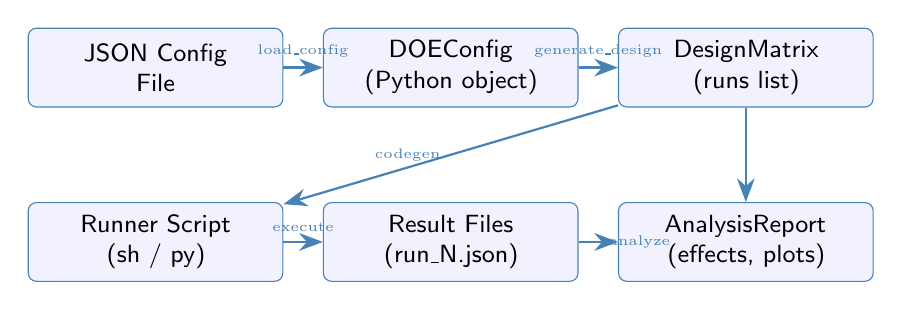
\begin{tikzpicture}[
  node distance=1.2cm and 0.5cm,
  box/.style={
    draw=steelblue, fill=blue!5, rounded corners=3pt,
    text width=3cm, minimum height=1cm, align=center,
    font=\small\sffamily
  },
  arr/.style={-{Stealth[length=3mm]}, thick, steelblue}
]
  \node[box] (config) {JSON Config\\File};
  \node[box, right=of config] (doeconfig) {DOEConfig\\(Python object)};
  \node[box, right=of doeconfig] (matrix) {DesignMatrix\\(runs list)};
  \node[box, below=of config] (script) {Runner Script\\(sh / py)};
  \node[box, below=of doeconfig] (results) {Result Files\\(run\_N.json)};
  \node[box, below=of matrix] (report) {AnalysisReport\\(effects, plots)};

  \draw[arr] (config) -- (doeconfig) node[midway,above,font=\tiny] {load\_config};
  \draw[arr] (doeconfig) -- (matrix) node[midway,above,font=\tiny] {generate\_design};
  \draw[arr] (matrix) -- (script) node[midway,left,font=\tiny] {codegen};
  \draw[arr] (script) -- (results) node[midway,above,font=\tiny] {execute};
  \draw[arr] (results) -- (report) node[midway,right,font=\tiny] {analyze};
  \draw[arr] (matrix) -- (report);
\end{tikzpicture}
\end{center}

\section{Where Files Go}

\begin{table}[H]
\centering
\caption{Output locations}
\begin{tabular}{@{}lll@{}}
\toprule
\textbf{What} & \textbf{Config Field} & \textbf{Default} \\
\midrule
Result JSON files & \texttt{settings.out\_directory} & \texttt{results} \\
Analysis plots, CSV & \texttt{settings.processed\_directory} & same as out\_directory \\
Runner script & \texttt{--output} flag & \texttt{run\_experiments.sh} \\
HTML report & \texttt{--output} flag on report & \texttt{report.html} \\
\bottomrule
\end{tabular}
\end{table}

\section{The Role of --seed}

The \texttt{--seed} flag controls randomization of run order. When you pass a seed to \texttt{doe generate}, runs within each block are shuffled using that seed. The purpose is twofold:

\begin{enumerate}
  \item \textbf{Randomization}: Shuffling run order guards against systematic time-dependent effects (e.g., a machine warming up during early runs).
  \item \textbf{Reproducibility}: The same seed always produces the same run order, so you can regenerate the exact same script later.
\end{enumerate}

For Latin Hypercube designs, the seed also controls the LHS sampling itself (via NumPy's random state), not just the run ordering.

\begin{warning}[Seed mismatch between generate and analyze]
The \texttt{analyze} command re-derives the design matrix by calling \texttt{generate\_design(cfg)} \emph{without} a seed argument. For designs where the seed only controls \emph{run order} (full factorial, PB, CCD, BB, fractional factorial), this means the analyze matrix has a different run order than the generated script---but the mapping from run IDs to factor values may differ. The result files are keyed by run ID (\texttt{run\_1.json}, \texttt{run\_2.json}, etc.), so the analyze command reads the correct data for each run ID regardless of ordering. For LHS designs, where the seed controls the actual sample points, not passing the same seed to analyze will produce a different design entirely. In practice, this means you should verify your results carefully when using LHS with a seed.
\end{warning}

\section{Why Analyze Re-derives the Design}

The \texttt{analyze} command does not read the generated runner script. Instead, it re-derives the design matrix from the configuration file by calling \texttt{generate\_design(cfg)}. This is by design: the config file is the single source of truth. The analyze command then loads result files from the output directory and matches them to the design matrix by run ID.

This architecture means:
\begin{itemize}
  \item You do not need to keep the runner script after execution.
  \item You can modify the config file's \texttt{out\_directory} or \texttt{processed\_directory} after running experiments and analyze will still work (use \texttt{--results-dir} to override).
  \item The config file must not be changed in ways that alter the design matrix (e.g., adding or removing factors, changing levels) between generation and analysis.
\end{itemize}


% ══════════════════════════════════════════════════════════════
\part{Configuration Reference}
% ══════════════════════════════════════════════════════════════

\chapter{The Configuration File}
\label{ch:config}

The configuration file is a JSON document that defines your entire experiment. This chapter documents every field in detail.

\section{Complete Anatomy}

A fully-specified configuration file has six top-level sections:

\begin{lstlisting}[language=json]
{
    "metadata":      { ... },
    "factors":       [ ... ],
    "fixed_factors": { ... },
    "responses":     [ ... ],
    "runner":        { ... },
    "settings":      { ... }
}
\end{lstlisting}

\section{The metadata Section}

\begin{table}[H]
\centering
\begin{tabular}{@{}lllp{5cm}@{}}
\toprule
\textbf{Field} & \textbf{Type} & \textbf{Default} & \textbf{Description} \\
\midrule
\texttt{name} & string & \texttt{""} & Human-readable experiment name \\
\texttt{description} & string & \texttt{""} & Longer description of the experiment \\
\bottomrule
\end{tabular}
\end{table}

Both fields are optional but recommended. They appear in \texttt{info} output, generated script headers, and the HTML report title.

\section{The factors Section}
\label{sec:factors}

The \texttt{factors} array defines the variables you want to study. Each element can be either a dictionary (modern format) or an array (legacy format).

\subsection{Modern Dictionary Format}

\begin{lstlisting}[language=json]
{
    "name": "temperature",
    "levels": ["150", "200"],
    "type": "continuous",
    "unit": "C",
    "description": "Reactor temperature"
}
\end{lstlisting}

\begin{table}[H]
\centering
\caption{Factor fields}
\begin{tabular}{@{}lllp{5cm}@{}}
\toprule
\textbf{Field} & \textbf{Type} & \textbf{Default} & \textbf{Description} \\
\midrule
\texttt{name} & string & (required) & Unique identifier for the factor \\
\texttt{levels} & array & (required) & At least 2 values; stored as strings \\
\texttt{type} & string & \texttt{"categorical"} & One of: \texttt{categorical}, \texttt{continuous}, \texttt{ordinal} \\
\texttt{unit} & string & \texttt{""} & Unit of measurement (display only) \\
\texttt{description} & string & \texttt{""} & Human-readable description \\
\bottomrule
\end{tabular}
\end{table}

\subsection{How Factor Types Affect Behavior}

The \texttt{type} field matters in two contexts:

\begin{enumerate}
  \item \textbf{Latin Hypercube sampling}: For \texttt{continuous} factors with 2 levels, LHS interpolates between the low and high values. For example, if levels are \texttt{["150", "200"]}, a sample at $x=0.3$ maps to $150 + 0.3 \times (200 - 150) = 165$. For \texttt{categorical} or \texttt{ordinal} factors, LHS bins the $[0,1]$ sample into discrete levels.
  \item \textbf{RSM encoding}: For \texttt{continuous} and \texttt{ordinal} factors, the RSM model normalizes values as $(v - \text{center}) / \text{half\_range}$. For \texttt{categorical} factors with two levels, it encodes as $-1$ and $+1$.
\end{enumerate}

For full factorial, Plackett--Burman, fractional factorial, CCD, and Box--Behnken designs, the type field has no effect on the generated design matrix---all runs use the exact level values specified.

\subsection{How Many Levels?}

\begin{table}[H]
\centering
\caption{Level requirements by design type}
\begin{tabular}{@{}ll@{}}
\toprule
\textbf{Design} & \textbf{Level Requirement} \\
\midrule
Full factorial & Any number $\geq 2$ per factor \\
Plackett--Burman & Exactly 2 per factor \\
Fractional factorial & Exactly 2 per factor \\
Latin Hypercube & Any number $\geq 2$ per factor \\
Central Composite (CCD) & Exactly 2 numeric levels per factor \\
Box--Behnken & Exactly 2 numeric levels per factor \\
\bottomrule
\end{tabular}
\end{table}

\begin{keypoint}[CCD and Box--Behnken generate intermediate values]
For CCD and Box--Behnken designs, you specify only the low and high levels (e.g., \texttt{["150", "200"]}). The tool automatically generates center points at $(150+200)/2 = 175$ and, for CCD, star (axial) points beyond the factorial range.
\end{keypoint}

\subsection{Legacy Array Format}

For backward compatibility, factors can also be specified as arrays:

\begin{lstlisting}[language=json]
"factors": [
    ["temperature", "low", "high"],
    ["pressure", "1", "5", "10"]
]
\end{lstlisting}

The first element is the factor name; the remaining elements are levels. Legacy-format factors default to \texttt{type="categorical"} with no unit or description.

\section{The responses Section}

\begin{lstlisting}[language=json]
"responses": [
    {"name": "yield",  "optimize": "maximize", "unit": "%",
     "description": "Product yield"},
    {"name": "cost",   "optimize": "minimize", "unit": "USD",
     "description": "Batch cost"}
]
\end{lstlisting}

\begin{table}[H]
\centering
\caption{Response fields}
\begin{tabular}{@{}lllp{5cm}@{}}
\toprule
\textbf{Field} & \textbf{Type} & \textbf{Default} & \textbf{Description} \\
\midrule
\texttt{name} & string & (required) & Must match the key in result JSON files \\
\texttt{optimize} & string & \texttt{"maximize"} & Either \texttt{maximize} or \texttt{minimize} \\
\texttt{unit} & string & \texttt{""} & Unit of measurement (display only) \\
\texttt{description} & string & \texttt{""} & Human-readable description \\
\bottomrule
\end{tabular}
\end{table}

\begin{keypoint}[What happens when responses is omitted]
If the \texttt{responses} array is empty or absent, the tool defaults to a single response named \texttt{"response"} with \texttt{optimize="maximize"}. Your test script must then produce JSON like \texttt{\{"response": 42.5\}}.
\end{keypoint}

For multi-response experiments, your test script must produce a JSON file with \emph{all} response keys:

\begin{lstlisting}[language=json]
{"yield": 87.3, "cost": 142.50, "purity": 99.1}
\end{lstlisting}

Responses can also be specified as simple strings (they default to \texttt{maximize}):

\begin{lstlisting}[language=json]
"responses": ["yield", "cost"]
\end{lstlisting}

\section{The runner Section}

\begin{lstlisting}[language=json]
"runner": {
    "arg_style": "double-dash",
    "result_file": "json"
}
\end{lstlisting}

\begin{table}[H]
\centering
\caption{Runner configuration fields}
\begin{tabular}{@{}lllp{5cm}@{}}
\toprule
\textbf{Field} & \textbf{Type} & \textbf{Default} & \textbf{Description} \\
\midrule
\texttt{arg\_style} & string & \texttt{"double-dash"} & How factors are passed to the test script \\
\texttt{result\_file} & string & \texttt{"json"} & Result file format (currently only JSON) \\
\bottomrule
\end{tabular}
\end{table}

\subsection{Argument Styles}

The \texttt{arg\_style} field controls how the generated runner script passes factor values to your test script. There are three options:

\begin{example}[double-dash (default)]
Each factor is passed as a named flag:
\begin{lstlisting}[language=bash]
./test_script.sh \
    --temperature "200" \
    --pressure "5" \
    --catalyst "1.5" \
    --duration "60" \
    --out "results/run_1.json"
\end{lstlisting}
Fixed factors are passed the same way, after the variable factors. The \texttt{--out} argument is always last.
\end{example}

\begin{example}[env]
Factors are exported as uppercase environment variables:
\begin{lstlisting}[language=bash]
export TEMPERATURE="200"
export PRESSURE="5"
export CATALYST="1.5"
export DURATION="60"
./test_script.sh --out "results/run_1.json"
\end{lstlisting}
The test script reads \texttt{\$TEMPERATURE}, \texttt{\$PRESSURE}, etc.\ from its environment. Only \texttt{--out} is passed as a command-line argument.
\end{example}

\begin{example}[positional]
Factor values are passed as positional arguments in order:
\begin{lstlisting}[language=bash]
./test_script.sh \
    "200" "5" "1.5" \
    "60" \
    --out "results/run_1.json"
\end{lstlisting}
Variable factors come first (in config order), then fixed factors, then \texttt{--out}.
\end{example}

\section{The settings Section}

\begin{lstlisting}[language=json]
"settings": {
    "operation": "full_factorial",
    "test_script": "examples/example_test_script.sh",
    "block_count": 1,
    "out_directory": "results",
    "processed_directory": "results/analysis",
    "lhs_samples": 0
}
\end{lstlisting}

\begin{table}[H]
\centering
\caption{Settings fields}
\begin{tabular}{@{}lllp{4.5cm}@{}}
\toprule
\textbf{Field} & \textbf{Type} & \textbf{Default} & \textbf{Description} \\
\midrule
\texttt{operation} & string & \texttt{"full\_factorial"} & Design type (see below) \\
\texttt{test\_script} & string & \texttt{""} & Path to test script \\
\texttt{block\_count} & int & \texttt{1} & Number of blocks (replications) \\
\texttt{out\_directory} & string & \texttt{""} & Where result files are stored \\
\texttt{processed\_directory} & string & \texttt{""} & Where plots and CSV go \\
\texttt{lhs\_samples} & int & \texttt{0} & Number of LHS samples (0 = auto) \\
\bottomrule
\end{tabular}
\end{table}

\subsection{Supported Operations}

The \texttt{operation} field must be one of these six values:

\begin{table}[H]
\centering
\begin{tabular}{@{}ll@{}}
\toprule
\textbf{Operation} & \textbf{Description} \\
\midrule
\texttt{full\_factorial} & All combinations of all factor levels \\
\texttt{fractional\_factorial} & A fraction of the full factorial ($2^{k-p}$) \\
\texttt{plackett\_burman} & Screening design for many factors \\
\texttt{latin\_hypercube} & Space-filling design for continuous factors \\
\texttt{central\_composite} & Circumscribed CCD with center + star points \\
\texttt{box\_behnken} & Three-level design without extreme corners \\
\bottomrule
\end{tabular}
\end{table}

\subsection{lhs\_samples}

For Latin Hypercube designs, \texttt{lhs\_samples} sets the number of sample points. When set to 0 (the default), the tool uses $\max(10,\; 2 \times n_{\text{factors}})$.

\section{The fixed\_factors Section}

\begin{lstlisting}[language=json]
"fixed_factors": {
    "duration": "60",
    "warmup-time": "3"
}
\end{lstlisting}

Fixed factors are key-value pairs passed to every experiment run. They are \emph{not} varied across runs. They are useful for parameters that you want to hold constant but still need to pass to the test script (e.g., a timeout, a warmup period, a database name).

\section{Legacy Format Support}

The tool supports two legacy features for backward compatibility:

\subsection{static\_settings}

Instead of \texttt{fixed\_factors}, older configs used \texttt{static\_settings}---an array of \texttt{"--key=value"} strings:

\begin{lstlisting}[language=json]
"static_settings": [
    "--duration=60",
    "--warmup-time=3"
]
\end{lstlisting}

The tool automatically strips the \texttt{--} prefix and splits on \texttt{=} to produce the equivalent \texttt{fixed\_factors} dictionary.

\subsection{Array-format factors}

As shown in Section~\ref{sec:factors}, factors can be arrays like \texttt{["temperature", "low", "high"]}. These are converted to \texttt{Factor} objects with default \texttt{type="categorical"}.

\section{Validation Rules}

When a configuration is loaded, the tool validates it and raises clear error messages for any problems. See Appendix~\ref{app:errors} for the complete list of error messages with causes and fixes.


% ──────────────────────────────────────────────────────────────
\chapter{Writing Test Scripts}
\label{ch:testscripts}

The test script is the program that actually runs your experiment. It receives factor values as input and writes a JSON result file as output. This chapter explains the protocol in detail.

\section{The Test Script Protocol}

Every test script must:

\begin{enumerate}
  \item \textbf{Receive factor values} via the mechanism specified by \texttt{runner.arg\_style} (command-line flags, environment variables, or positional arguments).
  \item \textbf{Run the experiment} using those factor values.
  \item \textbf{Write a JSON file} to the path specified by the \texttt{--out} argument containing at least the response key(s) defined in the configuration.
\end{enumerate}

\section{Bash Test Script (double-dash style)}

\begin{lstlisting}[language=bash]
#!/usr/bin/env bash
# test_script.sh -- example test script for DOE Helper Tool
# Receives factors as --name "value" arguments
# Must write JSON to the path given by --out

# Parse arguments
while [[ $# -gt 0 ]]; do
  case "$1" in
    --temperature) TEMPERATURE="$2"; shift 2;;
    --pressure)    PRESSURE="$2";    shift 2;;
    --catalyst)    CATALYST="$2";    shift 2;;
    --duration)    DURATION="$2";    shift 2;;
    --out)         OUT_FILE="$2";    shift 2;;
    *) echo "Unknown arg: $1"; exit 1;;
  esac
done

# Run the actual experiment here
# (replace with your real workload)
RESULT=$(run_my_experiment \
    --temp "$TEMPERATURE" \
    --press "$PRESSURE" \
    --cat "$CATALYST" \
    --dur "$DURATION")

# Write result JSON
echo "{\"response\": $RESULT}" > "$OUT_FILE"
\end{lstlisting}

\section{Bash Test Script (env style)}

\begin{lstlisting}[language=bash]
#!/usr/bin/env bash
# test_script_env.sh -- reads factors from environment

# Parse only the --out argument
OUT_FILE=""
while [[ $# -gt 0 ]]; do
  case "$1" in
    --out) OUT_FILE="$2"; shift 2;;
    *) shift;;
  esac
done

# Factors are in environment variables (uppercased)
echo "Temperature: $TEMPERATURE"
echo "Pressure: $PRESSURE"

RESULT=$(run_my_experiment)

echo "{\"response\": $RESULT}" > "$OUT_FILE"
\end{lstlisting}

\section{Python Test Script}

\begin{lstlisting}[language=python]
#!/usr/bin/env python3
"""test_script.py -- example Python test script"""

import argparse
import json

parser = argparse.ArgumentParser()
parser.add_argument("--temperature", required=True)
parser.add_argument("--pressure", required=True)
parser.add_argument("--catalyst", required=True)
parser.add_argument("--duration", default="60")
parser.add_argument("--out", required=True)
args = parser.parse_args()

# Run the experiment
result = run_experiment(
    temperature=float(args.temperature),
    pressure=float(args.pressure),
    catalyst=float(args.catalyst),
    duration=int(args.duration),
)

# Write result JSON
with open(args.out, "w") as f:
    json.dump({"response": result}, f)
\end{lstlisting}

\section{The Output JSON Format}

The test script must write a JSON object whose keys match the response names in your configuration. For a single response named \texttt{"response"}:

\begin{lstlisting}[language=json]
{"response": 87.3}
\end{lstlisting}

For multiple responses:

\begin{lstlisting}[language=json]
{
    "yield": 87.3,
    "purity": 99.1,
    "cost": 142.50
}
\end{lstlisting}

\begin{warning}[Key names must match exactly]
The keys in your result JSON must exactly match the \texttt{name} fields in your \texttt{responses} configuration. If your config has \texttt{"name": "yield"} but your script writes \texttt{"Yield"}, the analyze command will report ``Warning: response 'yield' missing'' and exclude those runs.
\end{warning}

\section{Handling Fixed Factors}

Fixed factors are passed to the test script in the same manner as variable factors (depending on \texttt{arg\_style}). Your test script should accept them as regular arguments. If you use \texttt{env} style, fixed factors are exported as uppercase environment variables.

\section{Error Handling}

When a test script fails (non-zero exit code), the runner script:
\begin{itemize}
  \item Prints an error message (e.g., \texttt{ERROR: Run 3 failed}).
  \item Records the failed run ID.
  \item Continues to the next run (does not abort the entire experiment).
  \item At the end, reports how many runs failed and exits with code~1.
\end{itemize}

The \texttt{analyze} command requires all result files to be present. If a run failed and its result file is missing, analyze will raise a \texttt{FileNotFoundError} listing the missing run IDs.

\section{Tips for Test Scripts}

\begin{itemize}
  \item \textbf{Warmup periods}: If your system needs warmup (e.g., JVM hot-start, database cache priming), include a warmup phase inside the test script before measuring the response.
  \item \textbf{Cleanup}: Clean up any temporary resources (temp files, database tables, containers) at the end of each run to avoid interference between runs.
  \item \textbf{Idempotency}: Design your test script so it can be run multiple times with the same inputs and produce the same output. The runner script's skip logic relies on result file existence, but if you need to re-run a specific run, simply delete its result file.
  \item \textbf{The --out argument}: Always the last argument passed by the runner. Your script must accept it and write the result JSON to that path.
\end{itemize}


% ══════════════════════════════════════════════════════════════
\part{Commands Reference}
% ══════════════════════════════════════════════════════════════

\chapter{The generate Command}
\label{ch:generate}

\section{Synopsis}

\begin{lstlisting}[language=bash]
doe generate --config FILE [--output PATH] [--format sh|py]
             [--seed INT] [--dry-run]
\end{lstlisting}

\section{Flags}

\begin{table}[H]
\centering
\caption{\texttt{generate} command flags}
\begin{tabular}{@{}lllp{4.5cm}@{}}
\toprule
\textbf{Flag} & \textbf{Type} & \textbf{Default} & \textbf{Description} \\
\midrule
\texttt{--config} & path & (required) & Path to JSON configuration file \\
\texttt{--output} & path & \texttt{run\_experiments.sh} & Output script path \\
\texttt{--format} & \texttt{sh}\,|\,\texttt{py} & \texttt{sh} & Script format \\
\texttt{--seed}   & integer & \texttt{None} & Random seed for run order \\
\texttt{--dry-run} & flag & \texttt{false} & Print design matrix only \\
\bottomrule
\end{tabular}
\end{table}

\section{What It Does}

The \texttt{generate} command:
\begin{enumerate}
  \item Loads and validates the configuration file.
  \item Generates the design matrix (calling \texttt{pyDOE3} for designs that require it).
  \item Applies blocking (replicating the base design \texttt{block\_count} times).
  \item Randomizes run order within each block using the provided seed.
  \item Renders the design into a runner script using the Jinja2 template.
  \item Makes the output file executable (\texttt{chmod +x}).
\end{enumerate}

\section{The --dry-run Flag}

When \texttt{--dry-run} is specified, the command prints the design matrix (same format as \texttt{doe info}) without writing any files:

\begin{lstlisting}[language=bash]
$ doe generate --config examples/example_config.json \
    --seed 42 --dry-run
Plan      : example experiment
Desc      : 3-factor 2-level full factorial example
Operation : full_factorial
Factors   : temperature, pressure, catalyst
Base runs : 8
Blocks    : 1
Total runs: 8
Responses : response [maximize]
Fixed     : duration=60

run_id  block_id  temperature  pressure  catalyst
------------------------------------------------------
1       1         high         low       B
2       1         low          high      A
3       1         high         high      B
...
\end{lstlisting}

This is useful for verifying the design and run order before committing to script generation.

\section{Generated Bash Script Structure}

The bash runner script (\texttt{--format sh}) has this structure:

\begin{enumerate}
  \item \textbf{Header comment}: Timestamp, operation type, total runs, and plan name.
  \item \textbf{Setup}: \texttt{set -uo pipefail} for safe error handling; \texttt{mkdir -p} for the output directory; an empty \texttt{FAILED\_RUNS} array.
  \item \textbf{Per-run blocks}: For each run, the script:
    \begin{itemize}
      \item Checks if the result file already exists (skip logic).
      \item Prints the run number, block ID, and factor values.
      \item Invokes the test script with the appropriate argument style.
      \item Captures failures and appends to \texttt{FAILED\_RUNS}.
    \end{itemize}
  \item \textbf{Summary}: Reports failed runs (if any) and exits with code~1 on failure, or prints a success message.
\end{enumerate}

\section{Generated Python Script Structure}

The Python runner script (\texttt{--format py}) has the same logic but uses Python syntax:

\begin{itemize}
  \item Runs are defined as a Python list of dictionaries.
  \item The test script is invoked via \texttt{subprocess.run()} with \texttt{check=True}.
  \item For \texttt{env} arg style, environment variables are set via the \texttt{env} parameter of \texttt{subprocess.run()}.
  \item For \texttt{positional} style, factor values are passed as list elements.
  \item Failed runs raise \texttt{CalledProcessError}, which is caught and logged.
\end{itemize}

\begin{example}[Generating a Python runner]
\begin{lstlisting}[language=bash]
$ doe generate --config examples/example_config.json \
    --output run_experiments.py --format py --seed 42
Generated 8 runs -> run_experiments.py
Run with: bash run_experiments.py
\end{lstlisting}
You can then run it with \texttt{python3 run\_experiments.py}.
\end{example}

\section{Skip Logic and Error Recovery}

Both generated script formats include skip logic: if a result file already exists for a given run, that run is skipped. This means:

\begin{itemize}
  \item \textbf{Safe re-runs}: If the script is interrupted (e.g., power failure, SSH disconnect), you can re-run it and it will pick up where it left off.
  \item \textbf{Selective re-runs}: To re-run a specific run, delete its result file (e.g., \texttt{rm results/run\_3.json}) and re-execute the script.
  \item \textbf{Failed runs}: Runs that fail (non-zero exit from test script) do \emph{not} produce a result file, so they will be retried on the next execution.
\end{itemize}


% ──────────────────────────────────────────────────────────────
\chapter{The analyze Command}
\label{ch:analyze}

\section{Synopsis}

\begin{lstlisting}[language=bash]
doe analyze --config FILE [--results-dir DIR]
            [--no-plots] [--csv DIR]
\end{lstlisting}

\section{Flags}

\begin{table}[H]
\centering
\caption{\texttt{analyze} command flags}
\begin{tabular}{@{}lllp{4.5cm}@{}}
\toprule
\textbf{Flag} & \textbf{Type} & \textbf{Default} & \textbf{Description} \\
\midrule
\texttt{--config} & path & (required) & Path to JSON configuration file \\
\texttt{--results-dir} & path & config's \texttt{out\_directory} & Override result file location \\
\texttt{--no-plots} & flag & \texttt{false} & Skip generating PNG plots \\
\texttt{--csv} & path & \texttt{None} & Export analysis to CSV files \\
\bottomrule
\end{tabular}
\end{table}

\section{What It Computes}

The \texttt{analyze} command performs three types of analysis for each response:

\subsection{Main Effects}

For each factor, the main effect is computed as:
\begin{itemize}
  \item \textbf{Two-level factors}: The difference between the mean response at the high level and the mean response at the low level ($\bar{y}_{\text{high}} - \bar{y}_{\text{low}}$).
  \item \textbf{Multi-level factors}: The difference between the maximum and minimum level means ($\max(\bar{y}_i) - \min(\bar{y}_i)$).
\end{itemize}

The standard error is computed as $\sqrt{s^2 / n}$ where $s^2$ is the pooled variance across all observations and $n$ is the total count.

For two-level factors, 95\% confidence intervals are computed using a two-sample $t$-test with pooled variance (requires \texttt{scipy}).

Percentage contribution is $|\text{effect}_i| / \sum |\text{effect}_j| \times 100$.

Effects are sorted by absolute magnitude (largest first).

\subsection{Interaction Effects}

For every pair of two-level factors, the interaction effect is computed by:
\begin{enumerate}
  \item Grouping runs into ``concordant'' (both factors at the same level---both high or both low) and ``discordant'' (factors at opposite levels).
  \item Computing the difference: $\bar{y}_{\text{concordant}} - \bar{y}_{\text{discordant}}$.
\end{enumerate}

Interactions are also sorted by absolute magnitude.

\subsection{Summary Statistics}

For each factor, at each level, the tool computes: count ($N$), mean, standard deviation, minimum, and maximum of the response values.

\section{Complete Annotated Output}

Here is the full output for a 3-factor full factorial experiment with 8 runs:

\begin{lstlisting}[language=bash]
=== Main Effects: response ===
Factor               Effect    Std Error   % Contribution
--------------------------------------------------------------
temperature          12.4500      1.2340           52.1%
pressure              7.8200      0.9870           32.7%
catalyst              3.6300      0.7650           15.2%
\end{lstlisting}

\begin{itemize}
  \item \textbf{Factor}: The factor name, sorted by absolute effect (largest first).
  \item \textbf{Effect}: The signed main effect. Positive means the response increases from level~0 to level~1 (alphabetically sorted).
  \item \textbf{Std Error}: Standard error of the mean across all observations of this factor.
  \item \textbf{\% Contribution}: This factor's share of the total absolute effect across all factors. Here, temperature accounts for 52.1\% of the total variation.
\end{itemize}

\begin{lstlisting}[language=bash]
=== Interaction Effects: response ===
Factor A             Factor B             Interaction
                                                      % Contribution
------------------------------------------------------------------------
temperature          pressure                  2.1500           58.9%
temperature          catalyst                  1.1200           30.7%
pressure             catalyst                  0.3800           10.4%
\end{lstlisting}

\begin{itemize}
  \item \textbf{Interaction}: The signed interaction effect. A positive value means the response is higher when both factors are at the same level (both high or both low) than when they are at opposite levels.
  \item \textbf{\% Contribution}: This interaction's share of the total absolute interaction effect.
\end{itemize}

\begin{lstlisting}[language=bash]
=== Summary Statistics: response ===

temperature:
  Level               N      Mean       Std       Min       Max
  ------------------------------------------------------------
  high                4   91.2000    3.4500   87.3000   95.1000
  low                 4   78.7500    2.8900   75.2000   82.3000
\end{lstlisting}

\begin{itemize}
  \item \textbf{N}: Number of runs at this level.
  \item \textbf{Mean}: Average response value at this level.
  \item \textbf{Std}: Sample standard deviation (using $n-1$ denominator).
  \item \textbf{Min/Max}: The range of response values observed at this level.
\end{itemize}

\section{Plots}

Unless \texttt{--no-plots} is specified, two PNG files are generated per response in the \texttt{processed\_directory}:

\begin{enumerate}
  \item \textbf{Pareto chart} (\texttt{pareto\_\{response\}.png}): Horizontal bar chart of absolute main effects, sorted largest to smallest, with a cumulative percentage line and an 80\% threshold marker.
  \item \textbf{Main effects plot} (\texttt{main\_effects\_\{response\}.png}): One subplot per factor showing mean response at each level, connected by lines.
\end{enumerate}

\begin{keypoint}[Using --no-plots]
Use \texttt{--no-plots} when running in CI/CD pipelines, headless servers, or containers without a display. The analysis still runs; only the matplotlib-generated PNGs are skipped. If matplotlib is not installed, plots are skipped automatically with a warning.
\end{keypoint}

\section{CSV Export}

The \texttt{--csv DIR} flag creates two CSV files per response in the specified directory:

\begin{enumerate}
  \item \texttt{main\_effects\_\{response\}.csv} with columns:
    \begin{itemize}[nosep]
      \item \texttt{factor\_name}, \texttt{main\_effect}, \texttt{std\_error}, \texttt{pct\_contribution}, \texttt{ci\_low}, \texttt{ci\_high}
    \end{itemize}
  \item \texttt{summary\_stats\_\{response\}.csv} with columns:
    \begin{itemize}[nosep]
      \item \texttt{factor}, \texttt{level}, \texttt{n}, \texttt{mean}, \texttt{std}, \texttt{min}, \texttt{max}
    \end{itemize}
\end{enumerate}

\begin{example}[Exporting CSV files]
\begin{lstlisting}[language=bash]
$ doe analyze --config examples/example_config.json \
    --csv csv_output/
...
CSV exported: csv_output/main_effects_response.csv
CSV exported: csv_output/summary_stats_response.csv
\end{lstlisting}
\end{example}


% ──────────────────────────────────────────────────────────────
\chapter{The optimize Command}
\label{ch:optimize}

\section{Synopsis}

\begin{lstlisting}[language=bash]
doe optimize --config FILE [--results-dir DIR]
             [--response NAME]
\end{lstlisting}

\section{Flags}

\begin{table}[H]
\centering
\caption{\texttt{optimize} command flags}
\begin{tabular}{@{}lllp{4.5cm}@{}}
\toprule
\textbf{Flag} & \textbf{Type} & \textbf{Default} & \textbf{Description} \\
\midrule
\texttt{--config} & path & (required) & Path to JSON configuration file \\
\texttt{--results-dir} & path & config's \texttt{out\_directory} & Override result file location \\
\texttt{--response} & string & all responses & Optimize for a single response \\
\bottomrule
\end{tabular}
\end{table}

\section{What It Does}

For each response (or the one specified by \texttt{--response}), the optimize command performs three analyses:

\begin{enumerate}
  \item \textbf{Best observed run}: Finds the run with the best response value (maximum for \texttt{maximize}, minimum for \texttt{minimize}), and prints its factor settings and value.
  \item \textbf{RSM linear model}: Fits a linear regression model (Response Surface Model) using least-squares. Reports the model coefficients, $R^2$ value, and the predicted optimum (the observed factor combination that the model predicts gives the best response).
  \item \textbf{Factor importance}: Ranks factors by absolute main effect, showing each factor's effect magnitude and percentage contribution.
\end{enumerate}

\section{Complete Annotated Output}

\begin{lstlisting}[language=bash]
=== Optimization: yield ===
Direction: maximize

Best observed run: #7
  temperature = 200
  pressure = 6
  catalyst = 2.0
  Value: 94.5

RSM Model (linear, R^2 = 0.87):
  Coefficients:
    intercept:  +82.3500
    temperature:  +6.2250
    pressure:  +3.8100
    catalyst:  +1.9400
  Predicted optimum:
    temperature = 200
    pressure = 6
    catalyst = 2.0
    Predicted value: 94.3250

Factor importance:
  1. temperature  (effect: 12.5, contribution: 52.0%)
  2. pressure  (effect: 7.6, contribution: 31.7%)
  3. catalyst  (effect: 3.9, contribution: 16.3%)
\end{lstlisting}

\subsection{Understanding the Output}

\begin{itemize}
  \item \textbf{Best observed run}: The run with the highest (or lowest, for minimize) actual measured value. This is a fact---it tells you which combination performed best in your experiment.
  \item \textbf{RSM Model}: A linear regression fit to all the data. The coefficients tell you how much each factor contributes to the predicted response per coded unit change. The intercept is the grand mean. A positive coefficient for \texttt{temperature} means higher temperature predicts higher yield.
  \item \textbf{$R^2$}: The coefficient of determination. Values near 1.0 mean the linear model fits the data well. Values below 0.7 suggest the relationship may be nonlinear or there is substantial noise.
  \item \textbf{Predicted optimum}: The factor combination (from among the observed runs) that the fitted model predicts gives the best response. This may differ from the best observed run if the model smooths out noise.
  \item \textbf{Factor importance}: Same as the main effects from \texttt{analyze}, ranked by absolute effect.
\end{itemize}

\begin{keypoint}[When $R^2$ is low]
A low $R^2$ (below 0.7) means the linear model does not capture the relationship well. This could mean:
\begin{itemize}[nosep]
  \item The relationship is nonlinear---consider using a CCD or Box--Behnken design and fitting a quadratic model.
  \item There is significant noise---consider adding blocks (replications) to average out variability.
  \item Important factors are missing from the model.
\end{itemize}
The best observed run is still valid regardless of $R^2$; it is the model predictions that become unreliable.
\end{keypoint}

\section{Optimizing a Single Response}

In a multi-response experiment, use \texttt{--response} to focus on one response:

\begin{lstlisting}[language=bash]
$ doe optimize --config reactor_config.json \
    --response yield
\end{lstlisting}

Without \texttt{--response}, the command prints optimization results for every response defined in the config.


% ──────────────────────────────────────────────────────────────
\chapter{The info Command}
\label{ch:info}

\section{Synopsis}

\begin{lstlisting}[language=bash]
doe info --config FILE
\end{lstlisting}

\section{What It Shows}

The \texttt{info} command loads the configuration with \texttt{strict=False} and displays:

\begin{itemize}
  \item Plan name and description (from metadata).
  \item Operation type.
  \item Factor names.
  \item Number of base runs, blocks, and total runs.
  \item Response names with optimization direction and units.
  \item Fixed factor values.
  \item The complete design matrix (run ID, block ID, and factor values for every run).
\end{itemize}

\section{Why strict=False?}

With \texttt{strict=False}, the config loader skips the check for whether \texttt{test\_script} exists on disk. This means you can use \texttt{info} to preview a design \emph{before} you have written your test script, or when sharing a config file between machines where the test script is at different paths.

\begin{example}[Previewing a design]
\begin{lstlisting}[language=bash]
$ doe info --config examples/reactor_config.json
Plan      : Chemical Reactor Optimization
Desc      : Box-Behnken design to optimize yield and
            purity of a batch reactor process
Operation : box_behnken
Factors   : temperature, pressure, catalyst
Base runs : 15
Blocks    : 1
Total runs: 15
Responses : yield [maximize] (%), purity [maximize] (%),
            cost [minimize] (USD)
Fixed     : reaction_time=60, stirring_speed=300

run_id  block_id  temperature  pressure  catalyst
------------------------------------------------------
1       1         150          2         1.25
2       1         200          2         1.25
3       1         150          6         1.25
...
\end{lstlisting}
\end{example}

This is the fastest way to verify your configuration and see how many runs will be required before committing to an experiment.


% ──────────────────────────────────────────────────────────────
\chapter{The report Command}
\label{ch:report}

\section{Synopsis}

\begin{lstlisting}[language=bash]
doe report --config FILE [--results-dir DIR]
           [--output PATH]
\end{lstlisting}

\section{Flags}

\begin{table}[H]
\centering
\caption{\texttt{report} command flags}
\begin{tabular}{@{}lllp{4.5cm}@{}}
\toprule
\textbf{Flag} & \textbf{Type} & \textbf{Default} & \textbf{Description} \\
\midrule
\texttt{--config} & path & (required) & Path to JSON configuration file \\
\texttt{--results-dir} & path & config's \texttt{out\_directory} & Override result file location \\
\texttt{--output} & path & \texttt{report.html} & Output HTML file path \\
\bottomrule
\end{tabular}
\end{table}

\section{What the HTML Report Contains}

The generated HTML report is a single self-contained file with no external CSS or JavaScript dependencies. It contains:

\begin{enumerate}
  \item \textbf{Header}: Experiment name, description, and generation timestamp.
  \item \textbf{Design Summary} (collapsible): Operation type, number of factors, total runs, blocks, and a table of factor details (name, type, levels, unit).
  \item \textbf{Results per response} (collapsible): For each response:
    \begin{itemize}[nosep]
      \item Main effects table (factor, effect, std error, 95\% CI, \% contribution).
      \item Interaction effects table (if applicable).
      \item Summary statistics tables (one per factor).
      \item Embedded Pareto chart (PNG encoded as base64 data URI).
      \item Embedded main effects plot (PNG encoded as base64 data URI).
    \end{itemize}
  \item \textbf{Design Matrix} (collapsed by default): The full run table showing all factor values.
  \item \textbf{Footer}: ``Generated by DOE Helper Tool.''
\end{enumerate}

\section{Self-Contained Design}

The report uses \texttt{<details>} / \texttt{<summary>} HTML elements for collapsible sections. Plot images are embedded directly as base64-encoded PNGs inside \texttt{<img>} tags, so the file can be emailed, uploaded to a wiki, or opened offline without any missing dependencies.

\begin{example}[Generating and sharing a report]
\begin{lstlisting}[language=bash]
$ doe report --config examples/reactor_config.json \
    --output reactor_report.html
HTML report written to: reactor_report.html

# Share via email, open in any browser
$ open reactor_report.html     # macOS
$ xdg-open reactor_report.html # Linux
\end{lstlisting}
\end{example}


% ══════════════════════════════════════════════════════════════
\part{Design Types in Practice}
% ══════════════════════════════════════════════════════════════

\chapter{Choosing and Using Each Design Type}
\label{ch:designtypes}

This chapter provides practical guidance for each of the six supported design types: what it is, when to use it, how to configure it, and how many runs it requires.

\section{Full Factorial}

\subsection{Overview}

A full factorial design tests \emph{every} combination of factor levels. For $k$ factors with $l_1, l_2, \ldots, l_k$ levels respectively, the number of base runs is $\prod_{i=1}^{k} l_i$.

\subsection{Requirements}
\begin{itemize}[nosep]
  \item Each factor must have at least 2 levels.
  \item No constraint on factor types (categorical, continuous, ordinal all work).
  \item No external library needed (\texttt{pyDOE3} is not used).
\end{itemize}

\subsection{Number of Runs}

\begin{table}[H]
\centering
\begin{tabular}{@{}lll@{}}
\toprule
\textbf{Factors} & \textbf{Levels} & \textbf{Base Runs} \\
\midrule
2 & 2 each & $2^2 = 4$ \\
3 & 2 each & $2^3 = 8$ \\
4 & 2 each & $2^4 = 16$ \\
3 & 3 each & $3^3 = 27$ \\
2 & 2 and 3 & $2 \times 3 = 6$ \\
\bottomrule
\end{tabular}
\end{table}

\subsection{Config Snippet}

\begin{lstlisting}[language=json]
{
    "factors": [
        {"name": "A", "levels": ["low", "high"]},
        {"name": "B", "levels": ["low", "high"]},
        {"name": "C", "levels": ["low", "high"]}
    ],
    "settings": {"operation": "full_factorial"}
}
\end{lstlisting}

\subsection{When to Use}

Use full factorial when you have few factors (2--4) and can afford the number of runs. It provides complete information about all main effects and all interactions. It is the gold standard when resources allow.

\begin{warning}[Exponential growth]
A full factorial with 7 two-level factors requires $2^7 = 128$ base runs. With 3 blocks, that is 384 runs. If each run takes 10 minutes, the experiment takes over 60 hours. Consider screening designs (PB or fractional factorial) when you have many factors.
\end{warning}

\section{Fractional Factorial}

\subsection{Overview}

A fractional factorial tests a carefully chosen \emph{subset} of the full factorial. The tool generates a $2^{k-p}$ Resolution~III design, where $k$ is the number of factors and $p$ is determined automatically to minimize the number of runs while still estimating main effects.

\subsection{Requirements}
\begin{itemize}[nosep]
  \item Each factor must have \textbf{exactly 2 levels}.
  \item Requires \texttt{pyDOE3}.
\end{itemize}

\subsection{Number of Runs}

The number of base runs depends on the number of factors and the resolution. The tool computes the smallest $k$ base factors such that $k$ plus all interactions of those base factors covers all $n$ factors:

\begin{table}[H]
\centering
\begin{tabular}{@{}ll@{}}
\toprule
\textbf{Factors ($n$)} & \textbf{Typical Base Runs} \\
\midrule
3 & 4 \\
4--7 & 8 \\
8--15 & 16 \\
\bottomrule
\end{tabular}
\end{table}

\subsection{Config Snippet}

\begin{lstlisting}[language=json]
{
    "factors": [
        {"name": "A", "levels": ["low", "high"]},
        {"name": "B", "levels": ["low", "high"]},
        {"name": "C", "levels": ["low", "high"]},
        {"name": "D", "levels": ["low", "high"]},
        {"name": "E", "levels": ["low", "high"]}
    ],
    "settings": {"operation": "fractional_factorial"}
}
\end{lstlisting}

\subsection{When to Use}

Use fractional factorial when you have 4--15 two-level factors and want to estimate main effects with fewer runs than a full factorial. Be aware that some higher-order interactions will be aliased (confounded) with main effects due to the resolution trade-off.

\section{Plackett--Burman}

\subsection{Overview}

Plackett--Burman (PB) designs are screening designs that can test $N-1$ factors in $N$ runs (where $N$ is a multiple of 4). They are highly efficient for identifying which factors matter, but they cannot estimate interactions.

\subsection{Requirements}
\begin{itemize}[nosep]
  \item Each factor must have \textbf{exactly 2 levels}.
  \item Requires \texttt{pyDOE3}.
\end{itemize}

\subsection{Number of Runs}

The number of base runs is the smallest multiple of 4 that is $\geq n + 1$:

\begin{table}[H]
\centering
\begin{tabular}{@{}ll@{}}
\toprule
\textbf{Factors} & \textbf{Base Runs} \\
\midrule
2--3 & 4 \\
4--7 & 8 \\
8--11 & 12 \\
12--15 & 16 \\
16--19 & 20 \\
\bottomrule
\end{tabular}
\end{table}

\subsection{Config Snippet}

\begin{lstlisting}[language=json]
{
    "factors": [
        {"name": "threads",           "levels": ["1", "4"]},
        {"name": "memory_block_size", "levels": ["1K", "16K"]},
        {"name": "memory_scope_type", "levels": ["global", "local"]},
        {"name": "memory_access_mode","levels": ["seq", "rnd"]},
        {"name": "memory_oper",       "levels": ["read", "write"]},
        {"name": "rand_type",         "levels": ["special", "uniform"]}
    ],
    "settings": {"operation": "plackett_burman"}
}
\end{lstlisting}

\subsection{When to Use}

Use PB designs for initial screening when you have 4 or more factors and want to quickly identify the ``vital few'' that have the largest effects. Follow up with a more detailed design (full factorial or CCD) on the important factors only.

\section{Latin Hypercube}

\subsection{Overview}

Latin Hypercube Sampling (LHS) is a space-filling design that distributes sample points evenly across the factor space. Unlike factorial designs, it does not test specific level combinations but instead samples continuously within the factor ranges.

\subsection{Requirements}
\begin{itemize}[nosep]
  \item Each factor must have at least 2 levels.
  \item For continuous factors with 2 levels, LHS interpolates between the low and high values. For categorical factors, LHS bins the sample into discrete levels.
  \item Requires \texttt{pyDOE3}.
\end{itemize}

\subsection{Number of Runs}

The number of base runs is set by \texttt{lhs\_samples} in the config. If set to 0 (the default), the tool uses $\max(10,\; 2 \times n_{\text{factors}})$. The ``maximin'' criterion is used to maximize the minimum distance between sample points.

\subsection{Config Snippet}

\begin{lstlisting}[language=json]
{
    "factors": [
        {"name": "temperature", "levels": ["150", "200"],
         "type": "continuous"},
        {"name": "pressure",    "levels": ["2", "10"],
         "type": "continuous"},
        {"name": "flow_rate",   "levels": ["5", "25"],
         "type": "continuous"}
    ],
    "settings": {
        "operation": "latin_hypercube",
        "lhs_samples": 20
    }
}
\end{lstlisting}

\subsection{When to Use}

Use LHS when you have continuous factors and want to explore the design space broadly without committing to a structured factorial design. LHS is particularly good for computer experiments (simulations) where there is no random error and you want to map the response surface with good coverage. It is also useful when the number of factors is large (10+) and factorial designs would require too many runs.

\section{Central Composite Design (CCD)}

\subsection{Overview}

A Central Composite Design adds star (axial) points and center points to a $2^k$ factorial design, enabling estimation of quadratic (curved) relationships. The tool generates a circumscribed CCD with orthogonal alpha values.

\subsection{Requirements}
\begin{itemize}[nosep]
  \item Each factor must have \textbf{exactly 2 numeric levels} (low and high).
  \item Levels must be parseable as floating-point numbers.
  \item Requires \texttt{pyDOE3}.
\end{itemize}

\subsection{Number of Runs}

For $k$ factors: $2^k$ factorial points $+$ $2k$ star points $+$ center points (4 by default).

\begin{table}[H]
\centering
\begin{tabular}{@{}lllll@{}}
\toprule
\textbf{Factors} & \textbf{Factorial} & \textbf{Star} & \textbf{Center} & \textbf{Total} \\
\midrule
2 & 4 & 4 & 8 & 16 \\
3 & 8 & 6 & 8 & 22 \\
4 & 16 & 8 & 8 & 32 \\
5 & 32 & 10 & 8 & 50 \\
\bottomrule
\end{tabular}
\end{table}

The CCD implementation uses \texttt{pyDOE3.ccdesign()} with \texttt{center=(4,4)}, \texttt{alpha="orthogonal"}, and \texttt{face="circumscribed"}.

\subsection{Config Snippet}

\begin{lstlisting}[language=json]
{
    "factors": [
        {"name": "temperature", "levels": ["150", "200"],
         "type": "continuous", "unit": "C"},
        {"name": "pressure",    "levels": ["2", "6"],
         "type": "continuous", "unit": "bar"}
    ],
    "settings": {"operation": "central_composite"}
}
\end{lstlisting}

\subsection{When to Use}

Use CCD when you want to model curvature in the response surface---for example, when you suspect there is an optimal temperature between your low and high settings, not at either extreme. CCD is the standard choice for response surface methodology (RSM) and is best used after a screening experiment has identified 2--5 important factors.

\begin{keypoint}[Star points extend beyond the factor range]
In a circumscribed CCD, star points are located at a distance $\alpha$ from the center, which is \emph{outside} the factorial range defined by your low and high levels. For example, if your temperature range is 150--200, star points might be at 140 and 210. Make sure your experimental system can handle these extreme values.
\end{keypoint}

\section{Box--Behnken}

\subsection{Overview}

A Box--Behnken design is a three-level design that avoids the extreme corner points of a full factorial. Each run uses either the center value or the low/high value for each factor, but never the corners where all factors are simultaneously at their extremes.

\subsection{Requirements}
\begin{itemize}[nosep]
  \item \textbf{At least 3 factors}.
  \item Each factor must have \textbf{exactly 2 numeric levels} (low and high).
  \item Levels must be parseable as floating-point numbers.
  \item Requires \texttt{pyDOE3}.
\end{itemize}

\subsection{Number of Runs}

The number of base runs depends on the number of factors and includes 3 center points:

\begin{table}[H]
\centering
\begin{tabular}{@{}ll@{}}
\toprule
\textbf{Factors} & \textbf{Base Runs} \\
\midrule
3 & 15 \\
4 & 27 \\
5 & 46 \\
\bottomrule
\end{tabular}
\end{table}

\subsection{Config Snippet}

\begin{lstlisting}[language=json]
{
    "factors": [
        {"name": "temperature", "levels": ["150", "200"],
         "type": "continuous", "unit": "C"},
        {"name": "pressure",    "levels": ["2", "6"],
         "type": "continuous", "unit": "bar"},
        {"name": "catalyst",    "levels": ["0.5", "2.0"],
         "type": "continuous", "unit": "g/L"}
    ],
    "settings": {"operation": "box_behnken"}
}
\end{lstlisting}

\subsection{When to Use}

Use Box--Behnken when you need to model curvature (like CCD) but want to avoid extreme corner combinations that might be physically dangerous, expensive, or infeasible. Box--Behnken requires at least 3 factors. It is generally more efficient than CCD for 3--5 factors because it avoids star points that extend beyond the factor range.


% ──────────────────────────────────────────────────────────────
\chapter{Blocking and Randomization}
\label{ch:blocking}

\section{How Blocking Works}

The \texttt{block\_count} setting in the config specifies how many times the entire base design is replicated. Each replication is called a ``block.'' Blocking serves two purposes:

\begin{enumerate}
  \item \textbf{Replication}: Running the same factor combinations multiple times provides a measure of experimental error and increases statistical power.
  \item \textbf{Nuisance factor control}: If your experiment spans multiple days, machines, or batches, you can assign each block to a different day/machine/batch and later analyze whether the blocking factor introduced systematic variation.
\end{enumerate}

\subsection{Example: block\_count = 1}

With \texttt{block\_count = 1} and a $2^3$ full factorial, you get 8 runs, all in block~1:

\begin{lstlisting}[language=bash]
run_id  block_id  A     B     C
------------------------------------
1       1         low   low   A
2       1         low   low   B
3       1         low   high  A
...     1         ...   ...   ...
8       1         high  high  B
\end{lstlisting}

\subsection{Example: block\_count = 3}

With \texttt{block\_count = 3}, the same 8 combinations are replicated 3 times, giving 24 total runs:

\begin{lstlisting}[language=bash]
run_id  block_id  A     B     C
------------------------------------
1       1         high  low   B
2       1         low   high  A
...
8       1         low   low   A
9       2         low   high  B
10      2         high  low   A
...
16      2         high  high  B
17      3         high  high  A
18      3         low   low   B
...
24      3         low   high  A
\end{lstlisting}

\section{Within-Block Randomization}

Runs are randomized \emph{within} each block, not across blocks. This means:

\begin{itemize}
  \item All runs in block~1 are executed first (in random order), then all runs in block~2, and so on.
  \item The run IDs are assigned sequentially after randomization (run 1 through $N_{\text{total}}$).
  \item The same seed always produces the same shuffled order within each block.
\end{itemize}

\section{How --seed Controls Randomization}

The seed is used to initialize a \texttt{random.Random} instance that shuffles runs within each block. For LHS designs, the seed additionally controls the LHS sampling via NumPy's random state.

\begin{itemize}
  \item \texttt{--seed 42}: Deterministic, reproducible order.
  \item No \texttt{--seed}: The order depends on the design type. For full factorial, PB, FF, CCD, and BB, the base order from pyDOE3 (or itertools) is used without shuffling. For LHS, the NumPy default random state is used.
\end{itemize}

\section{When to Use Blocking}

\begin{itemize}
  \item \textbf{Multi-day experiments}: Run one block per day. If day-to-day variation exists, it will be captured in the blocking structure.
  \item \textbf{Multiple machines}: Run one block per machine to isolate machine-specific effects.
  \item \textbf{Statistical power}: Even without nuisance factors, replication reduces the standard error of your effect estimates by $\sqrt{n}$.
  \item \textbf{Confidence}: With 3 blocks, each factor combination is tested 3 times. The summary statistics (mean, std) become much more reliable.
\end{itemize}

\begin{keypoint}[Blocks multiply run count]
With $b$ blocks and a base design of $r$ runs, you execute $b \times r$ total runs. A 5-factor CCD with 3 blocks requires $50 \times 3 = 150$ runs. Plan your time budget accordingly.
\end{keypoint}


% ══════════════════════════════════════════════════════════════
\part{Tutorials}
% ══════════════════════════════════════════════════════════════

\chapter{Tutorial --- Database Performance Tuning}
\label{ch:tutorial-db}

This tutorial walks through a realistic three-phase experiment to optimize MySQL database throughput by tuning five server configuration parameters.

\section{The Problem}

You are a database administrator and want to maximize query throughput (queries per second) for a web application workload. You suspect that five MySQL configuration knobs affect performance:

\begin{enumerate}[nosep]
  \item \texttt{innodb\_buffer\_pool\_size}: 1\,GB vs.\ 8\,GB
  \item \texttt{innodb\_log\_file\_size}: 256\,MB vs.\ 2\,GB
  \item \texttt{max\_connections}: 100 vs.\ 500
  \item \texttt{query\_cache\_size}: 0 vs.\ 256\,MB
  \item \texttt{thread\_cache\_size}: 8 vs.\ 64
\end{enumerate}

You will use a three-phase approach: screen, refine, optimize.

\section{Phase 1: Plackett--Burman Screening}

With 5 factors, a PB design requires only 8 runs (the smallest multiple of 4 $\geq 6$).

\subsection{Configuration}

\begin{lstlisting}[language=json]
{
    "metadata": {
        "name": "MySQL PB Screening",
        "description": "Identify which of 5 MySQL knobs
                        affect throughput most"
    },
    "factors": [
        {"name": "buffer_pool_size",
         "levels": ["1G", "8G"]},
        {"name": "log_file_size",
         "levels": ["256M", "2G"]},
        {"name": "max_connections",
         "levels": ["100", "500"]},
        {"name": "query_cache_size",
         "levels": ["0", "256M"]},
        {"name": "thread_cache_size",
         "levels": ["8", "64"]}
    ],
    "responses": [
        {"name": "qps", "optimize": "maximize",
         "unit": "queries/sec"}
    ],
    "settings": {
        "operation": "plackett_burman",
        "test_script": "./mysql_bench.sh",
        "out_directory": "results/phase1",
        "processed_directory": "results/phase1/analysis",
        "block_count": 2
    }
}
\end{lstlisting}

We use \texttt{block\_count: 2} for replication, giving $8 \times 2 = 16$ total runs.

\subsection{Commands}

\begin{lstlisting}[language=bash]
# Preview the design
$ doe info --config mysql_pb.json

# Generate the runner script
$ doe generate --config mysql_pb.json \
    --output phase1_runner.sh --seed 123

# Execute the experiments
$ bash phase1_runner.sh

# Analyze results
$ doe analyze --config mysql_pb.json
\end{lstlisting}

\subsection{Interpreting the Results}

\begin{lstlisting}[language=bash]
=== Main Effects: qps ===
Factor               Effect    Std Error   % Contribution
--------------------------------------------------------------
buffer_pool_size     2450.0000    120.5000           48.2%
log_file_size        1380.0000     98.3000           27.2%
max_connections       720.0000     85.7000           14.2%
query_cache_size      340.0000     79.2000            6.7%
thread_cache_size     190.0000     76.1000            3.7%
\end{lstlisting}

The Pareto chart shows that \texttt{buffer\_pool\_size} and \texttt{log\_file\_size} together account for 75.4\% of the total effect. These are the ``vital few'' factors to investigate further.

\section{Phase 2: Full Factorial on Top 2 Factors}

Now focus on the two most impactful factors with a $2^2$ full factorial.

\subsection{Configuration}

\begin{lstlisting}[language=json]
{
    "metadata": {
        "name": "MySQL Full Factorial",
        "description": "Detailed study of buffer pool and
                        log file size"
    },
    "factors": [
        {"name": "buffer_pool_size",
         "levels": ["1G", "8G"]},
        {"name": "log_file_size",
         "levels": ["256M", "2G"]}
    ],
    "fixed_factors": {
        "max_connections": "300",
        "query_cache_size": "128M",
        "thread_cache_size": "32"
    },
    "responses": [
        {"name": "qps", "optimize": "maximize",
         "unit": "queries/sec"}
    ],
    "settings": {
        "operation": "full_factorial",
        "test_script": "./mysql_bench.sh",
        "out_directory": "results/phase2",
        "processed_directory": "results/phase2/analysis",
        "block_count": 3
    }
}
\end{lstlisting}

Notice that the three non-critical factors are now held constant as \texttt{fixed\_factors} at their midpoints.

\subsection{Commands and Analysis}

\begin{lstlisting}[language=bash]
$ doe generate --config mysql_ff.json \
    --output phase2_runner.sh --seed 456
Generated 12 runs -> phase2_runner.sh

$ bash phase2_runner.sh

$ doe analyze --config mysql_ff.json

=== Interaction Effects: qps ===
Factor A             Factor B             Interaction
                                                      % Contribution
------------------------------------------------------------------------
buffer_pool_size     log_file_size             850.0000          100.0%
\end{lstlisting}

The significant interaction tells us that the effect of increasing buffer pool size is larger when the log file size is also large. This synergy suggests both should be set high together.

\section{Phase 3: CCD Optimization}

For the final phase, use a Central Composite Design with numeric levels to find the precise optimum.

\subsection{Configuration}

\begin{lstlisting}[language=json]
{
    "metadata": {
        "name": "MySQL CCD Optimization",
        "description": "Find optimal buffer pool and
                        log file size settings"
    },
    "factors": [
        {"name": "buffer_pool_size_gb",
         "levels": ["2", "8"], "type": "continuous",
         "unit": "GB"},
        {"name": "log_file_size_mb",
         "levels": ["512", "2048"], "type": "continuous",
         "unit": "MB"}
    ],
    "fixed_factors": {
        "max_connections": "300",
        "query_cache_size": "128M",
        "thread_cache_size": "32"
    },
    "responses": [
        {"name": "qps", "optimize": "maximize",
         "unit": "queries/sec"}
    ],
    "settings": {
        "operation": "central_composite",
        "test_script": "./mysql_bench.sh",
        "out_directory": "results/phase3",
        "processed_directory": "results/phase3/analysis"
    }
}
\end{lstlisting}

\subsection{Commands}

\begin{lstlisting}[language=bash]
$ doe generate --config mysql_ccd.json \
    --output phase3_runner.sh --seed 789
Generated 16 runs -> phase3_runner.sh

$ bash phase3_runner.sh

$ doe optimize --config mysql_ccd.json

=== Optimization: qps ===
Direction: maximize

Best observed run: #12
  buffer_pool_size_gb = 8
  log_file_size_mb = 2048
  Value: 14520.0

RSM Model (linear, R^2 = 0.91):
  Coefficients:
    intercept:  +11250.0000
    buffer_pool_size_gb:  +1580.0000
    log_file_size_mb:  +920.0000
  Predicted optimum:
    buffer_pool_size_gb = 8
    log_file_size_mb = 2048
    Predicted value: 14350.0000

Factor importance:
  1. buffer_pool_size_gb  (effect: 3160.0,
     contribution: 63.2%)
  2. log_file_size_mb  (effect: 1840.0,
     contribution: 36.8%)
\end{lstlisting}

\subsection{Conclusion}

The three-phase approach took us from 5 unknown factors to a clear recommendation: set \texttt{buffer\_pool\_size} to 8\,GB and \texttt{log\_file\_size} to 2\,GB for maximum throughput. The RSM model with $R^2 = 0.91$ gives us high confidence in these settings.

Finally, generate a report to share with the team:

\begin{lstlisting}[language=bash]
$ doe report --config mysql_ccd.json \
    --output mysql_optimization_report.html
HTML report written to: mysql_optimization_report.html
\end{lstlisting}


% ──────────────────────────────────────────────────────────────
\chapter{Tutorial --- Chemical Reactor Optimization}
\label{ch:tutorial-reactor}

This tutorial uses the included \texttt{reactor\_config.json} example to optimize a chemical batch reactor with three continuous factors and three responses.

\section{The Problem}

You are optimizing a batch chemical reactor. Three process parameters can be adjusted:

\begin{enumerate}[nosep]
  \item \textbf{Temperature}: 150--200\,\textdegree C
  \item \textbf{Pressure}: 2--6\,bar
  \item \textbf{Catalyst concentration}: 0.5--2.0\,g/L
\end{enumerate}

Two parameters are held constant: reaction time (60\,min) and stirring speed (300\,rpm).

Three responses are measured:
\begin{itemize}[nosep]
  \item \textbf{Yield} (\%): maximize
  \item \textbf{Purity} (\%): maximize
  \item \textbf{Cost} (USD): minimize
\end{itemize}

\section{The Configuration}

\begin{lstlisting}[language=json]
{
    "metadata": {
        "name": "Chemical Reactor Optimization",
        "description": "Box-Behnken design to optimize
            yield and purity of a batch reactor process"
    },
    "factors": [
        {"name": "temperature", "levels": ["150", "200"],
         "type": "continuous", "unit": "C",
         "description": "Reactor temperature"},
        {"name": "pressure",    "levels": ["2", "6"],
         "type": "continuous", "unit": "bar",
         "description": "Operating pressure"},
        {"name": "catalyst",    "levels": ["0.5", "2.0"],
         "type": "continuous", "unit": "g/L",
         "description": "Catalyst concentration"}
    ],
    "fixed_factors": {
        "reaction_time": "60",
        "stirring_speed": "300"
    },
    "responses": [
        {"name": "yield",  "optimize": "maximize",
         "unit": "%"},
        {"name": "purity", "optimize": "maximize",
         "unit": "%"},
        {"name": "cost",   "optimize": "minimize",
         "unit": "USD"}
    ],
    "runner": {"arg_style": "double-dash"},
    "settings": {
        "block_count": 1,
        "test_script": "examples/reactor_sim.sh",
        "operation": "box_behnken",
        "processed_directory": "results/reactor/analysis",
        "out_directory": "results/reactor"
    }
}
\end{lstlisting}

\section{Why Box--Behnken?}

Box--Behnken is ideal here because:
\begin{itemize}
  \item We have exactly 3 continuous factors (BB requires at least 3).
  \item We want to model curvature but do not want extreme corner points (e.g., running at 200\,\textdegree C \emph{and} 6\,bar \emph{and} 2.0\,g/L catalyst simultaneously might be dangerous).
  \item BB generates only 15 runs (vs.\ 22 for CCD with 3 factors), saving time and materials.
\end{itemize}

\section{Step 1: Preview the Design}

\begin{lstlisting}[language=bash]
$ doe info --config examples/reactor_config.json
Plan      : Chemical Reactor Optimization
Desc      : Box-Behnken design to optimize yield and
            purity of a batch reactor process
Operation : box_behnken
Factors   : temperature, pressure, catalyst
Base runs : 15
Blocks    : 1
Total runs: 15
Responses : yield [maximize] (%), purity [maximize] (%),
            cost [minimize] (USD)
Fixed     : reaction_time=60, stirring_speed=300

run_id  block_id  temperature  pressure  catalyst
------------------------------------------------------
1       1         150          2         1.25
2       1         200          2         1.25
3       1         150          6         1.25
4       1         200          6         1.25
5       1         150          4         0.5
6       1         200          4         0.5
7       1         150          4         2
8       1         200          4         2
9       1         175          2         0.5
10      1         175          6         0.5
11      1         175          2         2
12      1         175          6         2
13      1         175          4         1.25
14      1         175          4         1.25
15      1         175          4         1.25
\end{lstlisting}

Notice the structure: runs 1--4 vary temperature and pressure while holding catalyst at center (1.25). Runs 5--8 vary temperature and catalyst while holding pressure at center (4). Runs 9--12 vary pressure and catalyst while holding temperature at center (175). Runs 13--15 are center points (all factors at their midpoints).

\section{Step 2: Generate and Execute}

\begin{lstlisting}[language=bash]
$ doe generate --config examples/reactor_config.json \
    --output reactor_runner.sh --seed 100
Generated 15 runs -> reactor_runner.sh

$ bash reactor_runner.sh
Starting 15 experiment runs...

=== Run 1 / 15 (Block 1) ===
  temperature = 175
  pressure = 4
  catalyst = 1.25
...
All runs complete. Results in: results/reactor
\end{lstlisting}

Each run produces a JSON file with three response keys:

\begin{lstlisting}[language=json]
{"yield": 82.4, "purity": 97.1, "cost": 185.20}
\end{lstlisting}

\section{Step 3: Analyze}

\begin{lstlisting}[language=bash]
$ doe analyze --config examples/reactor_config.json
\end{lstlisting}

The output now shows three separate analysis sections---one per response:

\begin{lstlisting}[language=bash]
=== Main Effects: yield ===
Factor               Effect    Std Error   % Contribution
--------------------------------------------------------------
temperature           8.5000      0.9200           45.7%
pressure              6.2000      0.8100           33.3%
catalyst              3.9000      0.7500           21.0%

=== Main Effects: purity ===
Factor               Effect    Std Error   % Contribution
--------------------------------------------------------------
catalyst              2.8000      0.3100           48.3%
temperature           1.9000      0.2800           32.8%
pressure              1.1000      0.2500           19.0%

=== Main Effects: cost ===
Factor               Effect    Std Error   % Contribution
--------------------------------------------------------------
temperature          25.0000      2.1000           50.0%
catalyst             15.5000      1.8000           31.0%
pressure              9.5000      1.5000           19.0%
\end{lstlisting}

\section{Step 4: Optimize}

\begin{lstlisting}[language=bash]
$ doe optimize --config examples/reactor_config.json

=== Optimization: yield ===
Direction: maximize
Best observed run: #4
  temperature = 200
  pressure = 6
  catalyst = 1.25
  Value: 94.5
...

=== Optimization: purity ===
Direction: maximize
Best observed run: #12
  temperature = 175
  pressure = 6
  catalyst = 2
  Value: 99.2
...

=== Optimization: cost ===
Direction: minimize
Best observed run: #5
  temperature = 150
  pressure = 4
  catalyst = 0.5
  Value: 125.30
...
\end{lstlisting}

\section{Multi-Response Trade-offs}

The optimization reveals a classic trade-off:
\begin{itemize}
  \item \textbf{Maximum yield} requires high temperature and high pressure.
  \item \textbf{Maximum purity} requires moderate temperature with high catalyst.
  \item \textbf{Minimum cost} requires low temperature and low catalyst.
\end{itemize}

You cannot simultaneously maximize yield, maximize purity, and minimize cost. The optimize command shows the best settings for each response independently. In practice, you would choose a compromise based on your priorities---for example, set temperature to 175 (moderate), pressure to 6 (high), and catalyst to 1.5 (medium-high) to get good yield and purity at an acceptable cost.

\begin{keypoint}[Using --response for focused optimization]
To focus on a single response:
\begin{lstlisting}[language=bash]
$ doe optimize --config examples/reactor_config.json \
    --response yield
\end{lstlisting}
This prints only the yield optimization, which is cleaner when you have decided which response to prioritize.
\end{keypoint}

\section{Step 5: Generate a Report}

\begin{lstlisting}[language=bash]
$ doe report --config examples/reactor_config.json \
    --output reactor_report.html
HTML report written to: reactor_report.html
\end{lstlisting}

The HTML report contains collapsible sections for each response, with embedded Pareto charts and main effects plots. The design matrix section (collapsed by default) shows all 15 runs with their Box--Behnken factor values.


% ══════════════════════════════════════════════════════════════
\appendix
% ══════════════════════════════════════════════════════════════

\chapter{Error Messages Reference}
\label{app:errors}

This appendix catalogs every error message the tool can produce, with the cause and the fix.

\section{Configuration Validation Errors}

These errors are raised by \texttt{config.py} during \texttt{load\_config()}.

\begin{longtable}{@{}p{5.5cm}p{5.5cm}p{5.5cm}@{}}
\toprule
\textbf{Error Message} & \textbf{Cause} & \textbf{Fix} \\
\midrule
\endhead

\texttt{Unsupported operation '\{op\}'. Choose from: [box\_behnken, central\_composite, fractional\_factorial, full\_factorial, latin\_hypercube, plackett\_burman]} &
The \texttt{settings.operation} value is not one of the six supported design types. &
Set \texttt{operation} to one of the six valid values listed in the error message. \\
\midrule

\texttt{At least one factor is required.} &
The \texttt{factors} array is empty or missing. &
Add at least one factor with a name and at least 2 levels. \\
\midrule

\texttt{Factor names must be unique, got: [\ldots]} &
Two or more factors have the same \texttt{name}. &
Give each factor a distinct name. \\
\midrule

\texttt{block\_count must be >= 1, got \{n\}} &
The \texttt{block\_count} is set to 0 or a negative number. &
Set \texttt{block\_count} to 1 or higher. \\
\midrule

\texttt{Plackett-Burman requires exactly 2 levels per factor, but factor '\{name\}' has \{n\}: [\ldots]} &
A PB design was requested but a factor has more (or fewer) than 2 levels. &
Ensure every factor has exactly 2 levels, or use a different design type. \\
\midrule

\texttt{Fractional factorial requires exactly 2 levels per factor, but factor '\{name\}' has \{n\}: [\ldots]} &
A fractional factorial was requested but a factor does not have exactly 2 levels. &
Set each factor to exactly 2 levels. \\
\midrule

\texttt{Central composite requires exactly 2 levels (low, high) per factor, but factor '\{name\}' has \{n\}: [\ldots]} &
A CCD was requested but a factor does not have exactly 2 levels. &
Set each factor to exactly 2 numeric levels. \\
\midrule

\texttt{Central composite requires numeric levels, but factor '\{name\}' has non-numeric levels: [\ldots]} &
A CCD was requested but a factor's levels cannot be parsed as floats. &
Use numeric values (e.g., \texttt{["150", "200"]}) for all factor levels. \\
\midrule

\texttt{Box-Behnken requires at least 3 factors, but only \{n\} were provided.} &
A BB design was requested with fewer than 3 factors. &
Add more factors or use a different design type (CCD for 2 factors). \\
\midrule

\texttt{Box-Behnken requires exactly 2 levels (low, high) per factor, but factor '\{name\}' has \{n\}: [\ldots]} &
A BB design was requested but a factor does not have exactly 2 levels. &
Set each factor to exactly 2 numeric levels. \\
\midrule

\texttt{Box-Behnken requires numeric levels, but factor '\{name\}' has non-numeric levels: [\ldots]} &
A BB design was requested but a factor's levels are not numeric. &
Use numeric values for all factor levels. \\
\midrule

\texttt{Response names must be unique, got: [\ldots]} &
Two or more responses have the same \texttt{name}. &
Give each response a distinct name. \\
\midrule

\texttt{Response '\{name\}' has invalid optimize='\{val\}'. Choose from: [maximize, minimize]} &
A response's \texttt{optimize} field is not \texttt{maximize} or \texttt{minimize}. &
Set \texttt{optimize} to either \texttt{"maximize"} or \texttt{"minimize"}. \\
\midrule

\texttt{runner.arg\_style '\{val\}' is invalid. Choose from: [double-dash, env, positional]} &
The \texttt{runner.arg\_style} field is not one of the three valid values. &
Set \texttt{arg\_style} to \texttt{"double-dash"}, \texttt{"env"}, or \texttt{"positional"}. \\
\midrule

\texttt{Factor must have a name and at least 2 levels: \{item\}} &
A factor dict is missing \texttt{name} or has fewer than 2 levels. &
Provide a \texttt{name} and at least 2 values in \texttt{levels}. \\
\midrule

\texttt{Factor must have a name and at least one level: \{item\}} &
A legacy-format factor array is empty or has only one element. &
Provide at least the name and one level value. \\

\bottomrule
\end{longtable}

\section{Runtime Errors}

\begin{longtable}{@{}p{5.5cm}p{5.5cm}p{5.5cm}@{}}
\toprule
\textbf{Error Message} & \textbf{Cause} & \textbf{Fix} \\
\midrule
\endhead

\texttt{pyDOE3 is required for \{design\} designs. Install it with: pip install pyDOE3} &
The \texttt{pyDOE3} package is not installed but is needed for the requested design type. &
Run \texttt{pip install pyDOE3}. \\
\midrule

\texttt{Missing result files for run IDs: [\ldots]. Expected in: \{dir\}} &
The \texttt{analyze}, \texttt{optimize}, or \texttt{report} command could not find one or more result JSON files. &
Ensure all experiment runs completed successfully. Check the output directory. Re-run failed runs by deleting their result files and re-executing the runner script. \\
\midrule

\texttt{Warning: response '\{name\}' missing in result files for run IDs: [\ldots]} &
Some result JSON files exist but do not contain the expected response key. &
Check that your test script writes the correct key name in the result JSON. \\
\midrule

\texttt{Warning: test\_script '\{path\}' does not exist.} &
During \texttt{generate} (strict mode), the test script path does not exist. &
Create the test script or update the path in the config. This is a warning, not a fatal error. \\

\bottomrule
\end{longtable}


% ──────────────────────────────────────────────────────────────
\chapter{Output File Formats}
\label{app:formats}

\section{Result JSON Files (Per-Run)}

Each experiment run produces a file named \texttt{run\_\{N\}.json} in the output directory. The file is a JSON object whose keys must match the response names in the configuration:

\begin{lstlisting}[language=json]
{"yield": 87.3, "purity": 99.1, "cost": 142.50}
\end{lstlisting}

For a single response named \texttt{"response"}:

\begin{lstlisting}[language=json]
{"response": 87.3}
\end{lstlisting}

The naming convention is \texttt{run\_\{run\_id\}.json} where \texttt{run\_id} is the sequential integer assigned during design generation.

\section{CSV Export Format}

The \texttt{--csv DIR} flag on the \texttt{analyze} command creates two files per response:

\subsection{main\_effects\_\{response\}.csv}

\begin{table}[H]
\centering
\begin{tabular}{@{}llllll@{}}
\toprule
\texttt{factor\_name} & \texttt{main\_effect} & \texttt{std\_error} & \texttt{pct\_contribution} & \texttt{ci\_low} & \texttt{ci\_high} \\
\midrule
temperature & 12.45 & 1.234 & 52.1 & 9.82 & 15.08 \\
pressure & 7.82 & 0.987 & 32.7 & 5.71 & 9.93 \\
\bottomrule
\end{tabular}
\end{table}

All values are floating-point numbers. \texttt{ci\_low} and \texttt{ci\_high} are 0.0 if confidence intervals could not be computed.

\subsection{summary\_stats\_\{response\}.csv}

\begin{table}[H]
\centering
\begin{tabular}{@{}lllllll@{}}
\toprule
\texttt{factor} & \texttt{level} & \texttt{n} & \texttt{mean} & \texttt{std} & \texttt{min} & \texttt{max} \\
\midrule
temperature & high & 4 & 91.2 & 3.45 & 87.3 & 95.1 \\
temperature & low & 4 & 78.75 & 2.89 & 75.2 & 82.3 \\
\bottomrule
\end{tabular}
\end{table}

\section{HTML Report Structure}

The HTML report is a single file with embedded CSS (no external stylesheets) and base64-encoded PNG images. The structure uses semantic HTML5:

\begin{itemize}[nosep]
  \item \texttt{<header>}: Title, description, timestamp.
  \item \texttt{<details>} sections for Design Summary, Results per response, and Design Matrix.
  \item \texttt{<table>} elements with CSS classes \texttt{info-table} and \texttt{data-table}.
  \item \texttt{<img>} tags with \texttt{data:image/png;base64,\ldots} source URIs.
  \item \texttt{<footer>}: ``Generated by DOE Helper Tool.''
\end{itemize}

\section{Plot PNG Files}

Two PNG files are generated per response in the \texttt{processed\_directory}:

\begin{table}[H]
\centering
\begin{tabular}{@{}ll@{}}
\toprule
\textbf{File Name} & \textbf{Content} \\
\midrule
\texttt{pareto\_\{response\}.png} & Horizontal bar chart of absolute main effects with cumulative \% line \\
\texttt{main\_effects\_\{response\}.png} & Subplot grid showing mean response per level per factor \\
\bottomrule
\end{tabular}
\end{table}

Both are rendered at 150\,DPI. Special characters in response names (\texttt{/}, spaces) are replaced with underscores in file names.


% ──────────────────────────────────────────────────────────────
\chapter{Configuration Examples}
\label{app:examples}

\section{Minimal Configuration}

The smallest valid configuration: two factors, full factorial, no metadata:

\begin{lstlisting}[language=json]
{
    "factors": [
        {"name": "A", "levels": ["0", "1"]},
        {"name": "B", "levels": ["0", "1"]}
    ],
    "settings": {
        "operation": "full_factorial",
        "test_script": "./test.sh",
        "out_directory": "results"
    }
}
\end{lstlisting}

This produces 4 runs. Responses default to a single response named \texttt{"response"} with \texttt{optimize="maximize"}. The runner section defaults to \texttt{arg\_style="double-dash"}.

\section{Full-Featured Configuration}

Every field specified:

\begin{lstlisting}[language=json]
{
    "metadata": {
        "name": "Comprehensive Experiment",
        "description": "Testing all configuration fields"
    },
    "factors": [
        {"name": "temperature", "levels": ["150", "200"],
         "type": "continuous", "unit": "C",
         "description": "Process temperature"},
        {"name": "pressure", "levels": ["2", "6"],
         "type": "continuous", "unit": "bar",
         "description": "Operating pressure"},
        {"name": "catalyst", "levels": ["0.5", "2.0"],
         "type": "continuous", "unit": "g/L",
         "description": "Catalyst concentration"}
    ],
    "fixed_factors": {
        "reaction_time": "60",
        "stirring_speed": "300"
    },
    "responses": [
        {"name": "yield", "optimize": "maximize",
         "unit": "%",
         "description": "Product yield percentage"},
        {"name": "purity", "optimize": "maximize",
         "unit": "%",
         "description": "Product purity"},
        {"name": "cost", "optimize": "minimize",
         "unit": "USD",
         "description": "Batch production cost"}
    ],
    "runner": {
        "arg_style": "double-dash",
        "result_file": "json"
    },
    "settings": {
        "block_count": 2,
        "test_script": "./run_experiment.sh",
        "operation": "box_behnken",
        "processed_directory": "output/analysis",
        "out_directory": "output/results",
        "lhs_samples": 0
    }
}
\end{lstlisting}

\section{Multi-Response Configuration}

An experiment measuring three responses simultaneously:

\begin{lstlisting}[language=json]
{
    "metadata": {
        "name": "Multi-Response Study"
    },
    "factors": [
        {"name": "speed",    "levels": ["100", "500"]},
        {"name": "feed",     "levels": ["0.1", "0.5"]},
        {"name": "depth",    "levels": ["1", "5"]}
    ],
    "responses": [
        {"name": "surface_roughness",
         "optimize": "minimize", "unit": "um"},
        {"name": "material_removal_rate",
         "optimize": "maximize", "unit": "mm3/min"},
        {"name": "tool_wear",
         "optimize": "minimize", "unit": "mm"}
    ],
    "settings": {
        "operation": "box_behnken",
        "test_script": "./machining_test.sh",
        "out_directory": "results/machining"
    }
}
\end{lstlisting}

Your test script must produce JSON with all three keys:

\begin{lstlisting}[language=json]
{
    "surface_roughness": 1.23,
    "material_removal_rate": 45.6,
    "tool_wear": 0.05
}
\end{lstlisting}

\section{Legacy Format Configuration}

Using the older \texttt{static\_settings} and array-format factors:

\begin{lstlisting}[language=json]
{
    "factors": [
        ["temperature", "low", "high"],
        ["pressure", "low", "high"],
        ["catalyst", "A", "B"]
    ],
    "static_settings": [
        "--duration=60",
        "--warmup-time=3"
    ],
    "settings": {
        "operation": "full_factorial",
        "test_script": "./test.sh",
        "out_directory": "results"
    }
}
\end{lstlisting}

This is equivalent to the modern format with:
\begin{itemize}[nosep]
  \item Factors as dictionaries with \texttt{type="categorical"}.
  \item \texttt{fixed\_factors: \{"duration": "60", "warmup-time": "3"\}}.
  \item Default single response named \texttt{"response"}.
\end{itemize}

The tool automatically converts the legacy format during loading, so all commands work identically.


% ──────────────────────────────────────────────────────────────
\backmatter

\chapter*{Index of Commands}
\addcontentsline{toc}{chapter}{Index of Commands}

\begin{description}[style=nextline, labelwidth=4cm]
  \item[\texttt{doe generate}] Generate experiment runner script from config. See Chapter~\ref{ch:generate}.
  \item[\texttt{doe analyze}] Compute main effects, interactions, and summary statistics. See Chapter~\ref{ch:analyze}.
  \item[\texttt{doe optimize}] Find optimal factor settings with RSM. See Chapter~\ref{ch:optimize}.
  \item[\texttt{doe info}] Preview design without generating files. See Chapter~\ref{ch:info}.
  \item[\texttt{doe report}] Generate self-contained HTML report. See Chapter~\ref{ch:report}.
\end{description}

\end{document}
